\documentclass[twoside]{book}

% Packages required by doxygen
\usepackage{fixltx2e}
\usepackage{calc}
\usepackage{doxygen}
\usepackage[export]{adjustbox} % also loads graphicx
\usepackage{graphicx}
\usepackage[utf8]{inputenc}
\usepackage{makeidx}
\usepackage{multicol}
\usepackage{multirow}
\PassOptionsToPackage{warn}{textcomp}
\usepackage{textcomp}
\usepackage[nointegrals]{wasysym}
\usepackage[table]{xcolor}

% Font selection
\usepackage[T1]{fontenc}
\usepackage[scaled=.90]{helvet}
\usepackage{courier}
\usepackage{amssymb}
\usepackage{sectsty}
\renewcommand{\familydefault}{\sfdefault}
\allsectionsfont{%
  \fontseries{bc}\selectfont%
  \color{darkgray}%
}
\renewcommand{\DoxyLabelFont}{%
  \fontseries{bc}\selectfont%
  \color{darkgray}%
}
\newcommand{\+}{\discretionary{\mbox{\scriptsize$\hookleftarrow$}}{}{}}

% Page & text layout
\usepackage{geometry}
\geometry{%
  a4paper,%
  top=2.5cm,%
  bottom=2.5cm,%
  left=2.5cm,%
  right=2.5cm%
}
\tolerance=750
\hfuzz=15pt
\hbadness=750
\setlength{\emergencystretch}{15pt}
\setlength{\parindent}{0cm}
\setlength{\parskip}{0.2cm}
\makeatletter
\renewcommand{\paragraph}{%
  \@startsection{paragraph}{4}{0ex}{-1.0ex}{1.0ex}{%
    \normalfont\normalsize\bfseries\SS@parafont%
  }%
}
\renewcommand{\subparagraph}{%
  \@startsection{subparagraph}{5}{0ex}{-1.0ex}{1.0ex}{%
    \normalfont\normalsize\bfseries\SS@subparafont%
  }%
}
\makeatother

% Headers & footers
\usepackage{fancyhdr}
\pagestyle{fancyplain}
\fancyhead[LE]{\fancyplain{}{\bfseries\thepage}}
\fancyhead[CE]{\fancyplain{}{}}
\fancyhead[RE]{\fancyplain{}{\bfseries\leftmark}}
\fancyhead[LO]{\fancyplain{}{\bfseries\rightmark}}
\fancyhead[CO]{\fancyplain{}{}}
\fancyhead[RO]{\fancyplain{}{\bfseries\thepage}}
\fancyfoot[LE]{\fancyplain{}{}}
\fancyfoot[CE]{\fancyplain{}{}}
\fancyfoot[RE]{\fancyplain{}{\bfseries\scriptsize Generated on Mon Jul 27 2015 11\+:36\+:06 for My Project by Doxygen }}
\fancyfoot[LO]{\fancyplain{}{\bfseries\scriptsize Generated on Mon Jul 27 2015 11\+:36\+:06 for My Project by Doxygen }}
\fancyfoot[CO]{\fancyplain{}{}}
\fancyfoot[RO]{\fancyplain{}{}}
\renewcommand{\footrulewidth}{0.4pt}
\renewcommand{\chaptermark}[1]{%
  \markboth{#1}{}%
}
\renewcommand{\sectionmark}[1]{%
  \markright{\thesection\ #1}%
}

% Indices & bibliography
\usepackage{natbib}
\usepackage[titles]{tocloft}
\setcounter{tocdepth}{3}
\setcounter{secnumdepth}{5}
\makeindex

% Custom commands
\newcommand{\clearemptydoublepage}{%
  \newpage{\pagestyle{empty}\cleardoublepage}%
}


%===== C O N T E N T S =====

\begin{document}

% Titlepage & ToC
\pagenumbering{roman}
\begin{titlepage}
\vspace*{7cm}
\begin{center}%
{\Large My Project }\\
\vspace*{1cm}
{\large Generated by Doxygen 1.8.10}\\
\vspace*{0.5cm}
{\small Mon Jul 27 2015 11:36:06}\\
\end{center}
\end{titlepage}
\clearemptydoublepage
\tableofcontents
\clearemptydoublepage
\pagenumbering{arabic}

%--- Begin generated contents ---
\chapter{Hierarchical Index}
\section{Class Hierarchy}
This inheritance list is sorted roughly, but not completely, alphabetically\+:\begin{DoxyCompactList}
\item \contentsline{section}{App\+Delegate()}{\pageref{category_app_delegate_07_08}}{}
\item $<$A\+V\+Capture\+Metadata\+Output\+Objects\+Delegate$>$\begin{DoxyCompactList}
\item \contentsline{section}{Scan\+View\+Controller()}{\pageref{category_scan_view_controller_07_08}}{}
\end{DoxyCompactList}
\item \contentsline{section}{Book\+Detail\+View\+Controller()}{\pageref{category_book_detail_view_controller_07_08}}{}
\item \contentsline{section}{Manual\+View\+Controller()}{\pageref{category_manual_view_controller_07_08}}{}
\item N\+S\+Object\begin{DoxyCompactList}
\item \contentsline{section}{Result}{\pageref{interface_result}}{}
\item \contentsline{section}{Save}{\pageref{interface_save}}{}
\item \contentsline{section}{Search}{\pageref{interface_search}}{}
\item \contentsline{section}{T\+F\+Hpple}{\pageref{interface_t_f_hpple}}{}
\item \contentsline{section}{T\+F\+Hpple\+Element}{\pageref{interface_t_f_hpple_element}}{}
\end{DoxyCompactList}
\item $<$N\+S\+X\+M\+L\+Parser\+Delegate$>$\begin{DoxyCompactList}
\item \contentsline{section}{Search}{\pageref{interface_search}}{}
\end{DoxyCompactList}
\item \contentsline{section}{Result\+Table\+View\+Controller()}{\pageref{category_result_table_view_controller_07_08}}{}
\item \contentsline{section}{Saved\+List\+Table\+View\+Controller()}{\pageref{category_saved_list_table_view_controller_07_08}}{}
\item \contentsline{section}{T\+F\+Hpple()}{\pageref{category_t_f_hpple_07_08}}{}
\item \contentsline{section}{T\+F\+Hpple\+Element()}{\pageref{category_t_f_hpple_element_07_08}}{}
\item $<$U\+I\+Application\+Delegate$>$\begin{DoxyCompactList}
\item \contentsline{section}{App\+Delegate}{\pageref{interface_app_delegate}}{}
\end{DoxyCompactList}
\item U\+I\+Responder\begin{DoxyCompactList}
\item \contentsline{section}{App\+Delegate}{\pageref{interface_app_delegate}}{}
\end{DoxyCompactList}
\item U\+I\+Table\+View\+Controller\begin{DoxyCompactList}
\item \contentsline{section}{Result\+Table\+View\+Controller}{\pageref{interface_result_table_view_controller}}{}
\item \contentsline{section}{Saved\+List\+Table\+View\+Controller}{\pageref{interface_saved_list_table_view_controller}}{}
\end{DoxyCompactList}
\item U\+I\+View\+Controller\begin{DoxyCompactList}
\item \contentsline{section}{Book\+Detail\+View\+Controller}{\pageref{interface_book_detail_view_controller}}{}
\item \contentsline{section}{Manual\+View\+Controller}{\pageref{interface_manual_view_controller}}{}
\item \contentsline{section}{Scan\+View\+Controller}{\pageref{interface_scan_view_controller}}{}
\item \contentsline{section}{web\+View\+Controller}{\pageref{interfaceweb_view_controller}}{}
\end{DoxyCompactList}
\item \contentsline{section}{web\+View\+Controller()}{\pageref{categoryweb_view_controller_07_08}}{}
\end{DoxyCompactList}

\chapter{Class Index}
\section{Class List}
Here are the classes, structs, unions and interfaces with brief descriptions\+:\begin{DoxyCompactList}
\item\contentsline{section}{\hyperlink{interface_app_delegate}{App\+Delegate} }{\pageref{interface_app_delegate}}{}
\item\contentsline{section}{\hyperlink{category_app_delegate_07_08}{App\+Delegate()} }{\pageref{category_app_delegate_07_08}}{}
\item\contentsline{section}{\hyperlink{interface_book_detail_view_controller}{Book\+Detail\+View\+Controller} }{\pageref{interface_book_detail_view_controller}}{}
\item\contentsline{section}{\hyperlink{category_book_detail_view_controller_07_08}{Book\+Detail\+View\+Controller()} }{\pageref{category_book_detail_view_controller_07_08}}{}
\item\contentsline{section}{\hyperlink{interface_manual_view_controller}{Manual\+View\+Controller} }{\pageref{interface_manual_view_controller}}{}
\item\contentsline{section}{\hyperlink{category_manual_view_controller_07_08}{Manual\+View\+Controller()} }{\pageref{category_manual_view_controller_07_08}}{}
\item\contentsline{section}{\hyperlink{interface_result}{Result} }{\pageref{interface_result}}{}
\item\contentsline{section}{\hyperlink{interface_result_table_view_controller}{Result\+Table\+View\+Controller} }{\pageref{interface_result_table_view_controller}}{}
\item\contentsline{section}{\hyperlink{category_result_table_view_controller_07_08}{Result\+Table\+View\+Controller()} }{\pageref{category_result_table_view_controller_07_08}}{}
\item\contentsline{section}{\hyperlink{interface_save}{Save} }{\pageref{interface_save}}{}
\item\contentsline{section}{\hyperlink{interface_saved_list_table_view_controller}{Saved\+List\+Table\+View\+Controller} }{\pageref{interface_saved_list_table_view_controller}}{}
\item\contentsline{section}{\hyperlink{category_saved_list_table_view_controller_07_08}{Saved\+List\+Table\+View\+Controller()} }{\pageref{category_saved_list_table_view_controller_07_08}}{}
\item\contentsline{section}{\hyperlink{interface_scan_view_controller}{Scan\+View\+Controller} }{\pageref{interface_scan_view_controller}}{}
\item\contentsline{section}{\hyperlink{category_scan_view_controller_07_08}{Scan\+View\+Controller()} }{\pageref{category_scan_view_controller_07_08}}{}
\item\contentsline{section}{\hyperlink{interface_search}{Search} }{\pageref{interface_search}}{}
\item\contentsline{section}{\hyperlink{interface_t_f_hpple}{T\+F\+Hpple} }{\pageref{interface_t_f_hpple}}{}
\item\contentsline{section}{\hyperlink{category_t_f_hpple_07_08}{T\+F\+Hpple()} }{\pageref{category_t_f_hpple_07_08}}{}
\item\contentsline{section}{\hyperlink{interface_t_f_hpple_element}{T\+F\+Hpple\+Element} }{\pageref{interface_t_f_hpple_element}}{}
\item\contentsline{section}{\hyperlink{category_t_f_hpple_element_07_08}{T\+F\+Hpple\+Element()} }{\pageref{category_t_f_hpple_element_07_08}}{}
\item\contentsline{section}{\hyperlink{interfaceweb_view_controller}{web\+View\+Controller} }{\pageref{interfaceweb_view_controller}}{}
\item\contentsline{section}{\hyperlink{categoryweb_view_controller_07_08}{web\+View\+Controller()} }{\pageref{categoryweb_view_controller_07_08}}{}
\end{DoxyCompactList}

\chapter{Class Documentation}
\hypertarget{interface_app_delegate}{}\section{App\+Delegate Class Reference}
\label{interface_app_delegate}\index{App\+Delegate@{App\+Delegate}}


{\ttfamily \#import $<$App\+Delegate.\+h$>$}



Inheritance diagram for App\+Delegate\+:
% FIG 0


Collaboration diagram for App\+Delegate\+:
% FIG 1
\subsection*{Properties}
\begin{DoxyCompactItemize}
\item 
U\+I\+Window $\ast$ \hyperlink{interface_app_delegate_acf48ac24125e688cac1a85445cd7fac2}{window}
\end{DoxyCompactItemize}


\subsection{Property Documentation}
\hypertarget{interface_app_delegate_acf48ac24125e688cac1a85445cd7fac2}{}\index{App\+Delegate@{App\+Delegate}!window@{window}}
\index{window@{window}!App\+Delegate@{App\+Delegate}}
\subsubsection[{window}]{\setlength{\rightskip}{0pt plus 5cm}-\/ (U\+I\+Window$\ast$) window\hspace{0.3cm}{\ttfamily [read]}, {\ttfamily [write]}, {\ttfamily [nonatomic]}, {\ttfamily [strong]}}\label{interface_app_delegate_acf48ac24125e688cac1a85445cd7fac2}


The documentation for this class was generated from the following file\+:\begin{DoxyCompactItemize}
\item 
Library\+Books/\hyperlink{_app_delegate_8h}{App\+Delegate.\+h}\end{DoxyCompactItemize}

\hypertarget{category_app_delegate_07_08}{}\section{App\+Delegate() Category Reference}
\label{category_app_delegate_07_08}\index{App\+Delegate()@{App\+Delegate()}}


The documentation for this category was generated from the following file\+:\begin{DoxyCompactItemize}
\item 
Library\+Books/\hyperlink{_app_delegate_8m}{App\+Delegate.\+m}\end{DoxyCompactItemize}

\section{Book\+Detail\+View\+Controller Class Reference}
\label{interface_book_detail_view_controller}\index{Book\+Detail\+View\+Controller@{Book\+Detail\+View\+Controller}}


Inheritance diagram for Book\+Detail\+View\+Controller\+:
\nopagebreak
\begin{figure}[H]
\begin{center}
\leavevmode
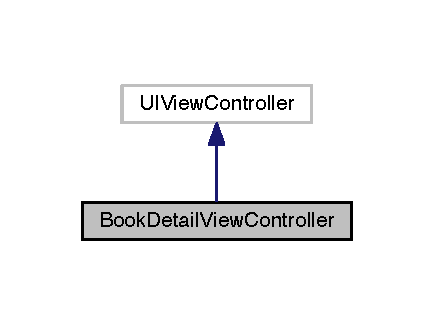
\includegraphics[width=208pt]{interface_book_detail_view_controller__inherit__graph}
\end{center}
\end{figure}


Collaboration diagram for Book\+Detail\+View\+Controller\+:
\nopagebreak
\begin{figure}[H]
\begin{center}
\leavevmode
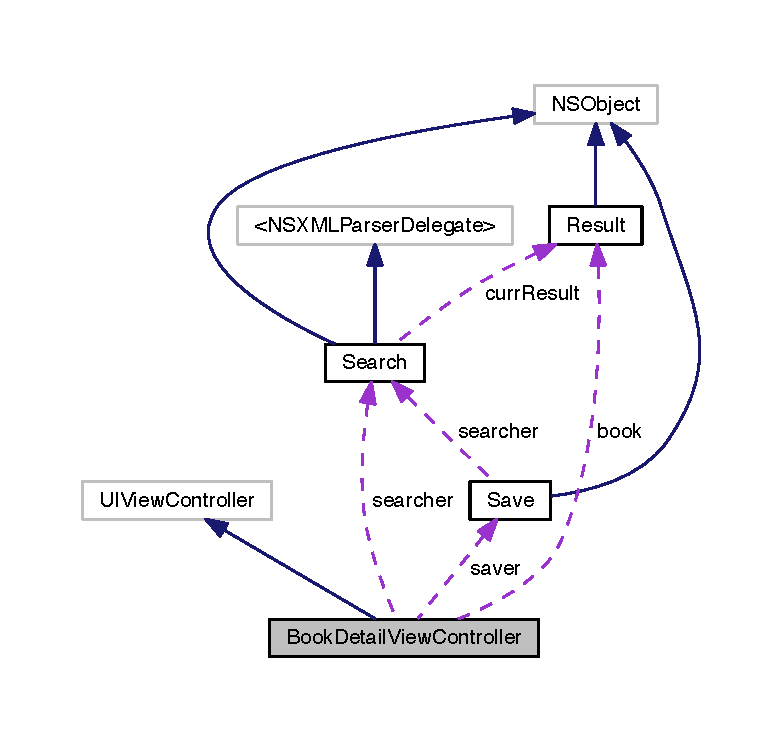
\includegraphics[width=350pt]{interface_book_detail_view_controller__coll__graph}
\end{center}
\end{figure}
\subsection*{Properties}
\begin{DoxyCompactItemize}
\item 
I\+B\+Outlet U\+I\+Image\+View $\ast$ {\bfseries book\+Image\+View}\label{interface_book_detail_view_controller_abc652edd9ccc4d9fcfb4509549ebbcca}

\item 
I\+B\+Outlet U\+I\+Label $\ast$ {\bfseries book\+Title}\label{interface_book_detail_view_controller_a8f8b751361cea806a31f828fd3b395a2}

\item 
I\+B\+Outlet U\+I\+Button $\ast$ {\bfseries call\+Num}\label{interface_book_detail_view_controller_aaf51d427a091cbbc8d56a583aae4c67f}

\item 
I\+B\+Outlet U\+I\+Activity\+Indicator\+View $\ast$ {\bfseries image\+Load\+Indicator}\label{interface_book_detail_view_controller_ae94c1e164a8be1c581349ed211421f18}

\item 
I\+B\+Outlet U\+I\+Label $\ast$ {\bfseries status}\label{interface_book_detail_view_controller_a7a734fdbd38ad55ff9dd7a1eac4f7851}

\item 
I\+B\+Outlet U\+I\+Text\+View $\ast$ {\bfseries desc\+Text\+View}\label{interface_book_detail_view_controller_a5041896b84e981aff8352686c6d163af}

\item 
I\+B\+Outlet U\+I\+Text\+View $\ast$ {\bfseries no\+Book\+View}\label{interface_book_detail_view_controller_a97334f844c3562b73bafd253a50ba060}

\item 
{\bf Result} $\ast$ {\bfseries book}\label{interface_book_detail_view_controller_afcef6fbafb9b021381b32df9a13d0b51}

\item 
N\+S\+String $\ast$ {\bfseries segged\+From}\label{interface_book_detail_view_controller_abd428e31e5786f92a707845b65f8307c}

\item 
N\+S\+String $\ast$ {\bfseries saved\+List\+Path}\label{interface_book_detail_view_controller_ab7004065d69e9415b54a4d8fb09669ec}

\item 
{\bf Save} $\ast$ {\bfseries saver}\label{interface_book_detail_view_controller_ac3455e9a6270af9f460694ec241af5ae}

\item 
{\bf Search} $\ast$ {\bfseries searcher}\label{interface_book_detail_view_controller_af7ab497759e614df06f71b732931a6ac}

\end{DoxyCompactItemize}


The documentation for this class was generated from the following file\+:\begin{DoxyCompactItemize}
\item 
Book\+Detail\+View\+Controller.\+h\end{DoxyCompactItemize}

\section{Book\+Detail\+View\+Controller() Category Reference}
\label{category_book_detail_view_controller_07_08}\index{Book\+Detail\+View\+Controller()@{Book\+Detail\+View\+Controller()}}


The documentation for this category was generated from the following file\+:\begin{DoxyCompactItemize}
\item 
Book\+Detail\+View\+Controller.\+m\end{DoxyCompactItemize}

\hypertarget{interface_manual_view_controller}{}\section{Manual\+View\+Controller Class Reference}
\label{interface_manual_view_controller}\index{Manual\+View\+Controller@{Manual\+View\+Controller}}


{\ttfamily \#import $<$Manual\+View\+Controller.\+h$>$}



Inheritance diagram for Manual\+View\+Controller\+:
% FIG 0


Collaboration diagram for Manual\+View\+Controller\+:
% FIG 1
\subsection*{Properties}
\begin{DoxyCompactItemize}
\item 
I\+B\+Outlet U\+I\+Text\+Field $\ast$ \hyperlink{interface_manual_view_controller_ac25b8675461f6b134f294d9d000d9acb}{query}
\item 
N\+S\+String $\ast$ \hyperlink{interface_manual_view_controller_a62433952d153e6ec83ab6b5abe6e9355}{type\+Selected}
\item 
I\+B\+Outlet U\+I\+Segmented\+Control $\ast$ \hyperlink{interface_manual_view_controller_a3ed5cace841a47be8974104d6c12d708}{type\+Control}
\item 
N\+S\+Mutable\+Array $\ast$ \hyperlink{interface_manual_view_controller_ae31761f23bddb440bbc90bb863860457}{results}
\item 
\hyperlink{interface_search}{Search} $\ast$ \hyperlink{interface_manual_view_controller_a0941a4f7be19492af2df58b8cd677f1e}{searcher}
\item 
I\+B\+Outlet U\+I\+Label $\ast$ \hyperlink{interface_manual_view_controller_afb8fb2ba7d2fb64adaee3d7e184210f1}{none\+Found\+Label}
\item 
B\+O\+O\+L \hyperlink{interface_manual_view_controller_a20df493383dde01e934348e4ccb33090}{is\+Sim\+Results}
\item 
I\+B\+Outlet U\+I\+Activity\+Indicator\+View $\ast$ \hyperlink{interface_manual_view_controller_ab7d5ed6694032c058f36de73cbbfffe1}{search\+Indicator}
\item 
I\+B\+Outlet U\+I\+Text\+View $\ast$ \hyperlink{interface_manual_view_controller_adefbb904483341f811d5997aaa1adedc}{gray\+Background}
\end{DoxyCompactItemize}


\subsection{Property Documentation}
\hypertarget{interface_manual_view_controller_adefbb904483341f811d5997aaa1adedc}{}\index{Manual\+View\+Controller@{Manual\+View\+Controller}!gray\+Background@{gray\+Background}}
\index{gray\+Background@{gray\+Background}!Manual\+View\+Controller@{Manual\+View\+Controller}}
\subsubsection[{gray\+Background}]{\setlength{\rightskip}{0pt plus 5cm}-\/ (I\+B\+Outlet U\+I\+Text\+View$\ast$) gray\+Background\hspace{0.3cm}{\ttfamily [read]}, {\ttfamily [write]}, {\ttfamily [nonatomic]}, {\ttfamily [weak]}}\label{interface_manual_view_controller_adefbb904483341f811d5997aaa1adedc}
\hypertarget{interface_manual_view_controller_a20df493383dde01e934348e4ccb33090}{}\index{Manual\+View\+Controller@{Manual\+View\+Controller}!is\+Sim\+Results@{is\+Sim\+Results}}
\index{is\+Sim\+Results@{is\+Sim\+Results}!Manual\+View\+Controller@{Manual\+View\+Controller}}
\subsubsection[{is\+Sim\+Results}]{\setlength{\rightskip}{0pt plus 5cm}-\/ (B\+O\+O\+L) is\+Sim\+Results\hspace{0.3cm}{\ttfamily [read]}, {\ttfamily [write]}, {\ttfamily [atomic]}}\label{interface_manual_view_controller_a20df493383dde01e934348e4ccb33090}
\hypertarget{interface_manual_view_controller_afb8fb2ba7d2fb64adaee3d7e184210f1}{}\index{Manual\+View\+Controller@{Manual\+View\+Controller}!none\+Found\+Label@{none\+Found\+Label}}
\index{none\+Found\+Label@{none\+Found\+Label}!Manual\+View\+Controller@{Manual\+View\+Controller}}
\subsubsection[{none\+Found\+Label}]{\setlength{\rightskip}{0pt plus 5cm}-\/ (I\+B\+Outlet U\+I\+Label$\ast$) none\+Found\+Label\hspace{0.3cm}{\ttfamily [read]}, {\ttfamily [write]}, {\ttfamily [nonatomic]}, {\ttfamily [weak]}}\label{interface_manual_view_controller_afb8fb2ba7d2fb64adaee3d7e184210f1}
\hypertarget{interface_manual_view_controller_ac25b8675461f6b134f294d9d000d9acb}{}\index{Manual\+View\+Controller@{Manual\+View\+Controller}!query@{query}}
\index{query@{query}!Manual\+View\+Controller@{Manual\+View\+Controller}}
\subsubsection[{query}]{\setlength{\rightskip}{0pt plus 5cm}-\/ (I\+B\+Outlet U\+I\+Text\+Field$\ast$) query\hspace{0.3cm}{\ttfamily [read]}, {\ttfamily [write]}, {\ttfamily [nonatomic]}, {\ttfamily [weak]}}\label{interface_manual_view_controller_ac25b8675461f6b134f294d9d000d9acb}
\hypertarget{interface_manual_view_controller_ae31761f23bddb440bbc90bb863860457}{}\index{Manual\+View\+Controller@{Manual\+View\+Controller}!results@{results}}
\index{results@{results}!Manual\+View\+Controller@{Manual\+View\+Controller}}
\subsubsection[{results}]{\setlength{\rightskip}{0pt plus 5cm}-\/ (N\+S\+Mutable\+Array$\ast$) results\hspace{0.3cm}{\ttfamily [read]}, {\ttfamily [write]}, {\ttfamily [atomic]}, {\ttfamily [strong]}}\label{interface_manual_view_controller_ae31761f23bddb440bbc90bb863860457}
\hypertarget{interface_manual_view_controller_a0941a4f7be19492af2df58b8cd677f1e}{}\index{Manual\+View\+Controller@{Manual\+View\+Controller}!searcher@{searcher}}
\index{searcher@{searcher}!Manual\+View\+Controller@{Manual\+View\+Controller}}
\subsubsection[{searcher}]{\setlength{\rightskip}{0pt plus 5cm}-\/ ({\bf Search}$\ast$) searcher\hspace{0.3cm}{\ttfamily [read]}, {\ttfamily [write]}, {\ttfamily [atomic]}, {\ttfamily [strong]}}\label{interface_manual_view_controller_a0941a4f7be19492af2df58b8cd677f1e}
\hypertarget{interface_manual_view_controller_ab7d5ed6694032c058f36de73cbbfffe1}{}\index{Manual\+View\+Controller@{Manual\+View\+Controller}!search\+Indicator@{search\+Indicator}}
\index{search\+Indicator@{search\+Indicator}!Manual\+View\+Controller@{Manual\+View\+Controller}}
\subsubsection[{search\+Indicator}]{\setlength{\rightskip}{0pt plus 5cm}-\/ (I\+B\+Outlet U\+I\+Activity\+Indicator\+View$\ast$) search\+Indicator\hspace{0.3cm}{\ttfamily [read]}, {\ttfamily [write]}, {\ttfamily [nonatomic]}, {\ttfamily [weak]}}\label{interface_manual_view_controller_ab7d5ed6694032c058f36de73cbbfffe1}
\hypertarget{interface_manual_view_controller_a3ed5cace841a47be8974104d6c12d708}{}\index{Manual\+View\+Controller@{Manual\+View\+Controller}!type\+Control@{type\+Control}}
\index{type\+Control@{type\+Control}!Manual\+View\+Controller@{Manual\+View\+Controller}}
\subsubsection[{type\+Control}]{\setlength{\rightskip}{0pt plus 5cm}-\/ (I\+B\+Outlet U\+I\+Segmented\+Control$\ast$) type\+Control\hspace{0.3cm}{\ttfamily [read]}, {\ttfamily [write]}, {\ttfamily [nonatomic]}, {\ttfamily [weak]}}\label{interface_manual_view_controller_a3ed5cace841a47be8974104d6c12d708}
\hypertarget{interface_manual_view_controller_a62433952d153e6ec83ab6b5abe6e9355}{}\index{Manual\+View\+Controller@{Manual\+View\+Controller}!type\+Selected@{type\+Selected}}
\index{type\+Selected@{type\+Selected}!Manual\+View\+Controller@{Manual\+View\+Controller}}
\subsubsection[{type\+Selected}]{\setlength{\rightskip}{0pt plus 5cm}-\/ (N\+S\+String$\ast$) type\+Selected\hspace{0.3cm}{\ttfamily [read]}, {\ttfamily [write]}, {\ttfamily [atomic]}, {\ttfamily [strong]}}\label{interface_manual_view_controller_a62433952d153e6ec83ab6b5abe6e9355}


The documentation for this class was generated from the following file\+:\begin{DoxyCompactItemize}
\item 
Library\+Books/\hyperlink{_manual_view_controller_8h}{Manual\+View\+Controller.\+h}\end{DoxyCompactItemize}

\section{Reachability Class Reference}
\label{interface_reachability}\index{Reachability@{Reachability}}


Inheritance diagram for Reachability\+:
\nopagebreak
\begin{figure}[H]
\begin{center}
\leavevmode
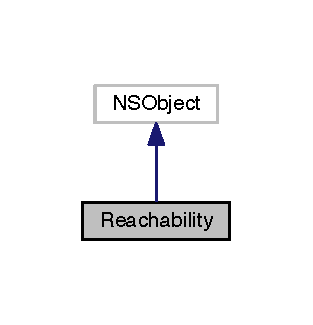
\includegraphics[width=150pt]{interface_reachability__inherit__graph}
\end{center}
\end{figure}


Collaboration diagram for Reachability\+:
\nopagebreak
\begin{figure}[H]
\begin{center}
\leavevmode
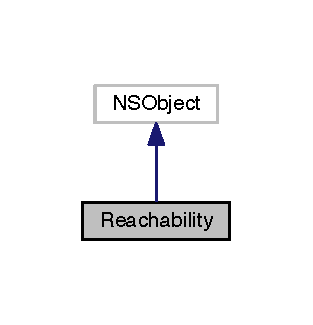
\includegraphics[width=150pt]{interface_reachability__coll__graph}
\end{center}
\end{figure}
\subsection*{Instance Methods}
\begin{DoxyCompactItemize}
\item 
(B\+O\+O\+L) -\/ {\bf start\+Notifier}
\item 
(void) -\/ {\bfseries stop\+Notifier}\label{interface_reachability_ab7907e9c8de0e4e15774e82c089e0b39}

\item 
(Network\+Status) -\/ {\bfseries current\+Reachability\+Status}\label{interface_reachability_a8396438436e7ff3770039fb527cd1d34}

\item 
(B\+O\+O\+L) -\/ {\bf connection\+Required}
\end{DoxyCompactItemize}
\subsection*{Class Methods}
\begin{DoxyCompactItemize}
\item 
(instancetype) + {\bf reachability\+With\+Host\+Name\+:}
\item 
(instancetype) + {\bf reachability\+With\+Address\+:}
\item 
(instancetype) + {\bf reachability\+For\+Internet\+Connection}
\item 
(instancetype) + {\bf reachability\+For\+Local\+Wi\+Fi}
\end{DoxyCompactItemize}


\subsection{Method Documentation}
\index{Reachability@{Reachability}!connection\+Required@{connection\+Required}}
\index{connection\+Required@{connection\+Required}!Reachability@{Reachability}}
\subsubsection[{connection\+Required()}]{\setlength{\rightskip}{0pt plus 5cm}-\/ (B\+O\+O\+L) connection\+Required 
\begin{DoxyParamCaption}
{}
\end{DoxyParamCaption}
}\label{interface_reachability_a731496d70dd8bfbd1b364df13cac2b4c}
W\+W\+A\+N may be available, but not active until a connection has been established. Wi\+Fi may require a connection for V\+P\+N on Demand. \index{Reachability@{Reachability}!reachability\+For\+Internet\+Connection@{reachability\+For\+Internet\+Connection}}
\index{reachability\+For\+Internet\+Connection@{reachability\+For\+Internet\+Connection}!Reachability@{Reachability}}
\subsubsection[{reachability\+For\+Internet\+Connection()}]{\setlength{\rightskip}{0pt plus 5cm}+ (instancetype) reachability\+For\+Internet\+Connection 
\begin{DoxyParamCaption}
{}
\end{DoxyParamCaption}
}\label{interface_reachability_aba5c531ea84e2f6ed6b1cb25f0c87404}
Checks whether the default route is available. Should be used by applications that do not connect to a particular host. \index{Reachability@{Reachability}!reachability\+For\+Local\+Wi\+Fi@{reachability\+For\+Local\+Wi\+Fi}}
\index{reachability\+For\+Local\+Wi\+Fi@{reachability\+For\+Local\+Wi\+Fi}!Reachability@{Reachability}}
\subsubsection[{reachability\+For\+Local\+Wi\+Fi()}]{\setlength{\rightskip}{0pt plus 5cm}+ (instancetype) reachability\+For\+Local\+Wi\+Fi 
\begin{DoxyParamCaption}
{}
\end{DoxyParamCaption}
}\label{interface_reachability_ad23f99b42e28143e250850196cccce70}
Checks whether a local Wi\+Fi connection is available. \index{Reachability@{Reachability}!reachability\+With\+Address\+:@{reachability\+With\+Address\+:}}
\index{reachability\+With\+Address\+:@{reachability\+With\+Address\+:}!Reachability@{Reachability}}
\subsubsection[{reachability\+With\+Address\+:(const struct sockaddr\+\_\+in $\ast$host\+Address)}]{\setlength{\rightskip}{0pt plus 5cm}+ (instancetype) reachability\+With\+Address\+: 
\begin{DoxyParamCaption}
\item[{(const struct sockaddr\+\_\+in $\ast$)}]{host\+Address}
\end{DoxyParamCaption}
}\label{interface_reachability_a10eca399184adb3a360296b236406257}
Use to check the reachability of a given I\+P address. \index{Reachability@{Reachability}!reachability\+With\+Host\+Name\+:@{reachability\+With\+Host\+Name\+:}}
\index{reachability\+With\+Host\+Name\+:@{reachability\+With\+Host\+Name\+:}!Reachability@{Reachability}}
\subsubsection[{reachability\+With\+Host\+Name\+:(\+N\+S\+String $\ast$host\+Name)}]{\setlength{\rightskip}{0pt plus 5cm}+ (instancetype) reachability\+With\+Host\+Name\+: 
\begin{DoxyParamCaption}
\item[{(N\+S\+String $\ast$)}]{host\+Name}
\end{DoxyParamCaption}
}\label{interface_reachability_a4e729345411817f077d873ee82c62a8a}
Use to check the reachability of a given host name. \index{Reachability@{Reachability}!start\+Notifier@{start\+Notifier}}
\index{start\+Notifier@{start\+Notifier}!Reachability@{Reachability}}
\subsubsection[{start\+Notifier()}]{\setlength{\rightskip}{0pt plus 5cm}-\/ (B\+O\+O\+L) start\+Notifier 
\begin{DoxyParamCaption}
{}
\end{DoxyParamCaption}
}\label{interface_reachability_ae20732960a222681fcc7caeb191158bc}
Start listening for reachability notifications on the current run loop. 

The documentation for this class was generated from the following files\+:\begin{DoxyCompactItemize}
\item 
Reachability.\+h\item 
Reachability.\+m\end{DoxyCompactItemize}

\hypertarget{interface_result}{}\section{Result Class Reference}
\label{interface_result}\index{Result@{Result}}


{\ttfamily \#import $<$Result.\+h$>$}



Inheritance diagram for Result\+:
% FIG 0


Collaboration diagram for Result\+:
% FIG 1
\subsection*{Properties}
\begin{DoxyCompactItemize}
\item 
N\+S\+String $\ast$ \hyperlink{interface_result_a221a82d22ef456d6a35cf6d74802b262}{title}
\item 
N\+S\+Mutable\+String $\ast$ \hyperlink{interface_result_ae0ee8bca9a5152da9dadaaa6e87df815}{full\+Title}
\item 
N\+S\+String $\ast$ \hyperlink{interface_result_a4762f86f65f843c100a26838b8b901d4}{sub\+Title}
\item 
N\+S\+String $\ast$ \hyperlink{interface_result_a986030e775d3d57737a1cbdd08415efc}{isbn}
\item 
N\+S\+String $\ast$ \hyperlink{interface_result_a5e884192413fb61453b6157c61580d37}{call\+Number}
\item 
N\+S\+String $\ast$ \hyperlink{interface_result_a5954ccfa6df362fda75ec5f276d2f16d}{bib\+Id}
\item 
N\+S\+String $\ast$ \hyperlink{interface_result_a0b86d59eecde1e63af6212fe878c9c2e}{image\+U\+R\+L}
\item 
N\+S\+String $\ast$ \hyperlink{interface_result_af3b3c099477d3b115685206a8431aae2}{location}
\item 
N\+S\+String $\ast$ \hyperlink{interface_result_ac14c9c42e2ab672d0ec95253f47f9a6b}{desc}
\end{DoxyCompactItemize}


\subsection{Property Documentation}
\hypertarget{interface_result_a5954ccfa6df362fda75ec5f276d2f16d}{}\index{Result@{Result}!bib\+Id@{bib\+Id}}
\index{bib\+Id@{bib\+Id}!Result@{Result}}
\subsubsection[{bib\+Id}]{\setlength{\rightskip}{0pt plus 5cm}-\/ (N\+S\+String$\ast$) bib\+Id\hspace{0.3cm}{\ttfamily [read]}, {\ttfamily [write]}, {\ttfamily [nonatomic]}, {\ttfamily [strong]}}\label{interface_result_a5954ccfa6df362fda75ec5f276d2f16d}
\hypertarget{interface_result_a5e884192413fb61453b6157c61580d37}{}\index{Result@{Result}!call\+Number@{call\+Number}}
\index{call\+Number@{call\+Number}!Result@{Result}}
\subsubsection[{call\+Number}]{\setlength{\rightskip}{0pt plus 5cm}-\/ (N\+S\+String$\ast$) call\+Number\hspace{0.3cm}{\ttfamily [read]}, {\ttfamily [write]}, {\ttfamily [nonatomic]}, {\ttfamily [strong]}}\label{interface_result_a5e884192413fb61453b6157c61580d37}
\hypertarget{interface_result_ac14c9c42e2ab672d0ec95253f47f9a6b}{}\index{Result@{Result}!desc@{desc}}
\index{desc@{desc}!Result@{Result}}
\subsubsection[{desc}]{\setlength{\rightskip}{0pt plus 5cm}-\/ (N\+S\+String$\ast$) desc\hspace{0.3cm}{\ttfamily [read]}, {\ttfamily [write]}, {\ttfamily [nonatomic]}, {\ttfamily [strong]}}\label{interface_result_ac14c9c42e2ab672d0ec95253f47f9a6b}
\hypertarget{interface_result_ae0ee8bca9a5152da9dadaaa6e87df815}{}\index{Result@{Result}!full\+Title@{full\+Title}}
\index{full\+Title@{full\+Title}!Result@{Result}}
\subsubsection[{full\+Title}]{\setlength{\rightskip}{0pt plus 5cm}-\/ (N\+S\+Mutable\+String$\ast$) full\+Title\hspace{0.3cm}{\ttfamily [read]}, {\ttfamily [write]}, {\ttfamily [nonatomic]}, {\ttfamily [strong]}}\label{interface_result_ae0ee8bca9a5152da9dadaaa6e87df815}
\hypertarget{interface_result_a0b86d59eecde1e63af6212fe878c9c2e}{}\index{Result@{Result}!image\+U\+R\+L@{image\+U\+R\+L}}
\index{image\+U\+R\+L@{image\+U\+R\+L}!Result@{Result}}
\subsubsection[{image\+U\+R\+L}]{\setlength{\rightskip}{0pt plus 5cm}-\/ (N\+S\+String$\ast$) image\+U\+R\+L\hspace{0.3cm}{\ttfamily [read]}, {\ttfamily [write]}, {\ttfamily [nonatomic]}, {\ttfamily [strong]}}\label{interface_result_a0b86d59eecde1e63af6212fe878c9c2e}
\hypertarget{interface_result_a986030e775d3d57737a1cbdd08415efc}{}\index{Result@{Result}!isbn@{isbn}}
\index{isbn@{isbn}!Result@{Result}}
\subsubsection[{isbn}]{\setlength{\rightskip}{0pt plus 5cm}-\/ (N\+S\+String$\ast$) isbn\hspace{0.3cm}{\ttfamily [read]}, {\ttfamily [write]}, {\ttfamily [nonatomic]}, {\ttfamily [strong]}}\label{interface_result_a986030e775d3d57737a1cbdd08415efc}
\hypertarget{interface_result_af3b3c099477d3b115685206a8431aae2}{}\index{Result@{Result}!location@{location}}
\index{location@{location}!Result@{Result}}
\subsubsection[{location}]{\setlength{\rightskip}{0pt plus 5cm}-\/ (N\+S\+String$\ast$) location\hspace{0.3cm}{\ttfamily [read]}, {\ttfamily [write]}, {\ttfamily [nonatomic]}, {\ttfamily [strong]}}\label{interface_result_af3b3c099477d3b115685206a8431aae2}
\hypertarget{interface_result_a4762f86f65f843c100a26838b8b901d4}{}\index{Result@{Result}!sub\+Title@{sub\+Title}}
\index{sub\+Title@{sub\+Title}!Result@{Result}}
\subsubsection[{sub\+Title}]{\setlength{\rightskip}{0pt plus 5cm}-\/ (N\+S\+String$\ast$) sub\+Title\hspace{0.3cm}{\ttfamily [read]}, {\ttfamily [write]}, {\ttfamily [nonatomic]}, {\ttfamily [strong]}}\label{interface_result_a4762f86f65f843c100a26838b8b901d4}
\hypertarget{interface_result_a221a82d22ef456d6a35cf6d74802b262}{}\index{Result@{Result}!title@{title}}
\index{title@{title}!Result@{Result}}
\subsubsection[{title}]{\setlength{\rightskip}{0pt plus 5cm}-\/ (N\+S\+String$\ast$) title\hspace{0.3cm}{\ttfamily [read]}, {\ttfamily [write]}, {\ttfamily [nonatomic]}, {\ttfamily [strong]}}\label{interface_result_a221a82d22ef456d6a35cf6d74802b262}


The documentation for this class was generated from the following file\+:\begin{DoxyCompactItemize}
\item 
Library\+Books/\hyperlink{_result_8h}{Result.\+h}\end{DoxyCompactItemize}

\section{Result\+Table\+View\+Controller Class Reference}
\label{interface_result_table_view_controller}\index{Result\+Table\+View\+Controller@{Result\+Table\+View\+Controller}}


Inheritance diagram for Result\+Table\+View\+Controller\+:
\nopagebreak
\begin{figure}[H]
\begin{center}
\leavevmode
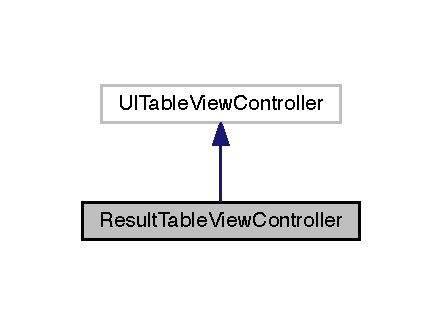
\includegraphics[width=212pt]{interface_result_table_view_controller__inherit__graph}
\end{center}
\end{figure}


Collaboration diagram for Result\+Table\+View\+Controller\+:
\nopagebreak
\begin{figure}[H]
\begin{center}
\leavevmode
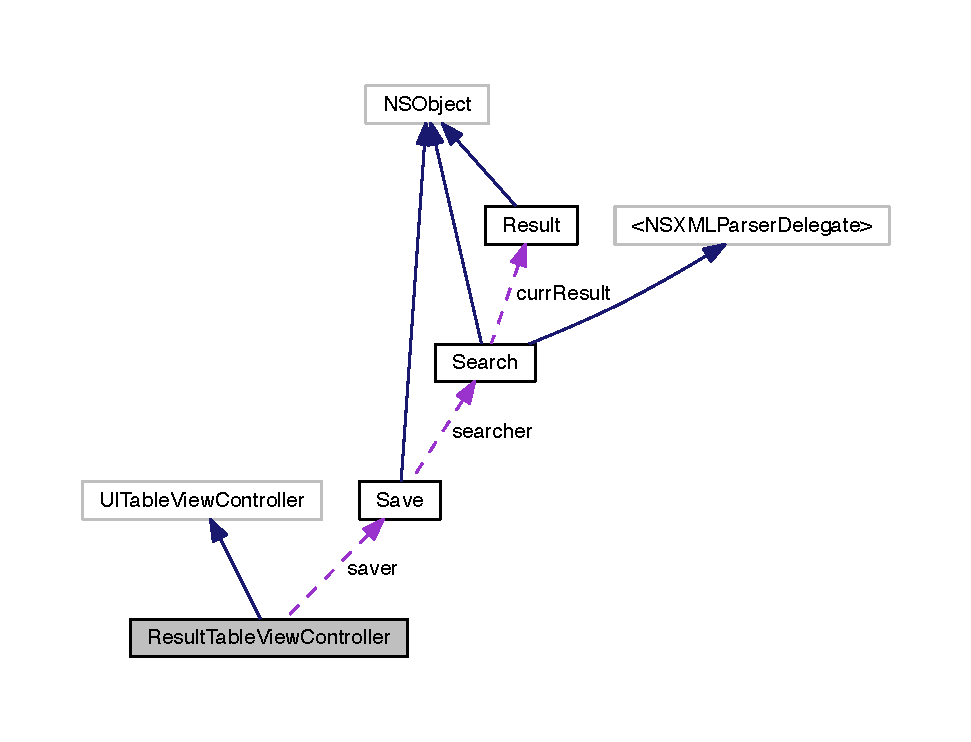
\includegraphics[width=350pt]{interface_result_table_view_controller__coll__graph}
\end{center}
\end{figure}
\subsection*{Properties}
\begin{DoxyCompactItemize}
\item 
U\+I\+View $\ast$ {\bfseries activity\+View}\label{interface_result_table_view_controller_a12b9e07c3d6de0154e485752f1779f84}

\item 
U\+I\+Alert\+View $\ast$ {\bfseries insert\+Name\+Alert}\label{interface_result_table_view_controller_ab06cf17fb0348c3cc4d8e268a5667c01}

\item 
N\+S\+Mutable\+Array $\ast$ {\bfseries results}\label{interface_result_table_view_controller_aac9b268204aac1044dc8e7dbe2927409}

\item 
{\bf Save} $\ast$ {\bfseries saver}\label{interface_result_table_view_controller_af56b1c31e591ad111fa3558a48e3fe6e}

\item 
N\+S\+String $\ast$ {\bfseries saved\+List\+Path}\label{interface_result_table_view_controller_a3bc64243af0d4d0b1ac9e4b4ce219a97}

\item 
B\+O\+O\+L {\bfseries is\+Sim\+Results}\label{interface_result_table_view_controller_ab58149d144b5844f39ce667aa900268f}

\item 
N\+S\+String $\ast$ {\bfseries query}\label{interface_result_table_view_controller_a05210302a3f2f54ca86edab3bdfb8d36}

\end{DoxyCompactItemize}


The documentation for this class was generated from the following file\+:\begin{DoxyCompactItemize}
\item 
Result\+Table\+View\+Controller.\+h\end{DoxyCompactItemize}

\hypertarget{category_result_table_view_controller_07_08}{}\section{Result\+Table\+View\+Controller() Category Reference}
\label{category_result_table_view_controller_07_08}\index{Result\+Table\+View\+Controller()@{Result\+Table\+View\+Controller()}}


The documentation for this category was generated from the following file\+:\begin{DoxyCompactItemize}
\item 
Library\+Books/\hyperlink{_result_table_view_controller_8m}{Result\+Table\+View\+Controller.\+m}\end{DoxyCompactItemize}

\section{Save Class Reference}
\label{interface_save}\index{Save@{Save}}


Inheritance diagram for Save\+:
\nopagebreak
\begin{figure}[H]
\begin{center}
\leavevmode
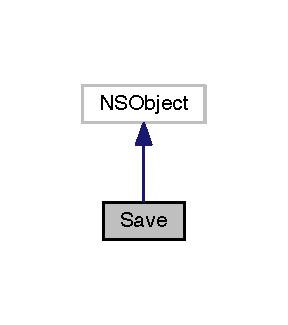
\includegraphics[width=138pt]{interface_save__inherit__graph}
\end{center}
\end{figure}


Collaboration diagram for Save\+:
\nopagebreak
\begin{figure}[H]
\begin{center}
\leavevmode
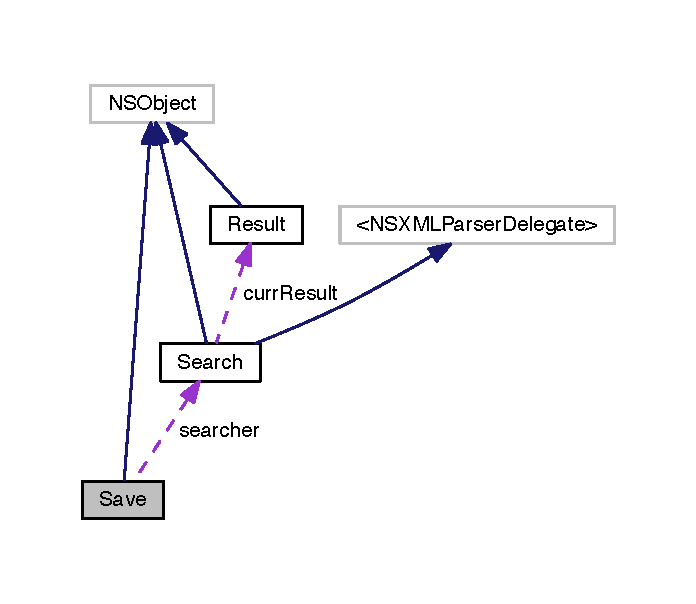
\includegraphics[width=334pt]{interface_save__coll__graph}
\end{center}
\end{figure}
\subsection*{Instance Methods}
\begin{DoxyCompactItemize}
\item 
(B\+O\+O\+L) -\/ {\bfseries save\+Items\+:::}\label{interface_save_a524d4353fa6366be4a70e2c5a1ec36ef}

\item 
(N\+S\+String $\ast$) -\/ {\bfseries load\+Saved\+Books\+File\+Path\+:}\label{interface_save_a73fcbcbfd899cca03c981caf11c4ed63}

\end{DoxyCompactItemize}
\subsection*{Properties}
\begin{DoxyCompactItemize}
\item 
{\bf Search} $\ast$ {\bfseries searcher}\label{interface_save_a159c85a712155c0e101efbb99e8a5c7e}

\end{DoxyCompactItemize}


The documentation for this class was generated from the following files\+:\begin{DoxyCompactItemize}
\item 
Save.\+h\item 
Save.\+m\end{DoxyCompactItemize}

\hypertarget{interface_saved_list_table_view_controller}{}\section{Saved\+List\+Table\+View\+Controller Class Reference}
\label{interface_saved_list_table_view_controller}\index{Saved\+List\+Table\+View\+Controller@{Saved\+List\+Table\+View\+Controller}}


{\ttfamily \#import $<$Saved\+List\+Table\+View\+Controller.\+h$>$}



Inheritance diagram for Saved\+List\+Table\+View\+Controller\+:
% FIG 0


Collaboration diagram for Saved\+List\+Table\+View\+Controller\+:
% FIG 1
\subsection*{Properties}
\begin{DoxyCompactItemize}
\item 
N\+S\+String $\ast$ \hyperlink{interface_saved_list_table_view_controller_a09a8915cb1823999764e52dfa661234c}{saved\+Books\+Path}
\item 
N\+S\+Dictionary $\ast$ \hyperlink{interface_saved_list_table_view_controller_a690c66541215851f8153757315f92dc6}{plist\+Main\+Dict}
\item 
N\+S\+Dictionary $\ast$ \hyperlink{interface_saved_list_table_view_controller_a9267936e6cbedae16a93f64b2f37912a}{curr\+Book}
\item 
N\+S\+Array $\ast$ \hyperlink{interface_saved_list_table_view_controller_a15911e64ef5023fe4f278081bcb5c7db}{plist\+Save\+Sections}
\item 
\hyperlink{interface_save}{Save} $\ast$ \hyperlink{interface_saved_list_table_view_controller_a666694532f2b5c88a4a74a7c4fff5fe2}{saver}
\end{DoxyCompactItemize}


\subsection{Property Documentation}
\hypertarget{interface_saved_list_table_view_controller_a9267936e6cbedae16a93f64b2f37912a}{}\index{Saved\+List\+Table\+View\+Controller@{Saved\+List\+Table\+View\+Controller}!curr\+Book@{curr\+Book}}
\index{curr\+Book@{curr\+Book}!Saved\+List\+Table\+View\+Controller@{Saved\+List\+Table\+View\+Controller}}
\subsubsection[{curr\+Book}]{\setlength{\rightskip}{0pt plus 5cm}-\/ (N\+S\+Dictionary$\ast$) curr\+Book\hspace{0.3cm}{\ttfamily [read]}, {\ttfamily [write]}, {\ttfamily [nonatomic]}, {\ttfamily [strong]}}\label{interface_saved_list_table_view_controller_a9267936e6cbedae16a93f64b2f37912a}
\hypertarget{interface_saved_list_table_view_controller_a690c66541215851f8153757315f92dc6}{}\index{Saved\+List\+Table\+View\+Controller@{Saved\+List\+Table\+View\+Controller}!plist\+Main\+Dict@{plist\+Main\+Dict}}
\index{plist\+Main\+Dict@{plist\+Main\+Dict}!Saved\+List\+Table\+View\+Controller@{Saved\+List\+Table\+View\+Controller}}
\subsubsection[{plist\+Main\+Dict}]{\setlength{\rightskip}{0pt plus 5cm}-\/ (N\+S\+Dictionary$\ast$) plist\+Main\+Dict\hspace{0.3cm}{\ttfamily [read]}, {\ttfamily [write]}, {\ttfamily [nonatomic]}, {\ttfamily [strong]}}\label{interface_saved_list_table_view_controller_a690c66541215851f8153757315f92dc6}
\hypertarget{interface_saved_list_table_view_controller_a15911e64ef5023fe4f278081bcb5c7db}{}\index{Saved\+List\+Table\+View\+Controller@{Saved\+List\+Table\+View\+Controller}!plist\+Save\+Sections@{plist\+Save\+Sections}}
\index{plist\+Save\+Sections@{plist\+Save\+Sections}!Saved\+List\+Table\+View\+Controller@{Saved\+List\+Table\+View\+Controller}}
\subsubsection[{plist\+Save\+Sections}]{\setlength{\rightskip}{0pt plus 5cm}-\/ (N\+S\+Array$\ast$) plist\+Save\+Sections\hspace{0.3cm}{\ttfamily [read]}, {\ttfamily [write]}, {\ttfamily [nonatomic]}, {\ttfamily [strong]}}\label{interface_saved_list_table_view_controller_a15911e64ef5023fe4f278081bcb5c7db}
\hypertarget{interface_saved_list_table_view_controller_a09a8915cb1823999764e52dfa661234c}{}\index{Saved\+List\+Table\+View\+Controller@{Saved\+List\+Table\+View\+Controller}!saved\+Books\+Path@{saved\+Books\+Path}}
\index{saved\+Books\+Path@{saved\+Books\+Path}!Saved\+List\+Table\+View\+Controller@{Saved\+List\+Table\+View\+Controller}}
\subsubsection[{saved\+Books\+Path}]{\setlength{\rightskip}{0pt plus 5cm}-\/ (N\+S\+String$\ast$) saved\+Books\+Path\hspace{0.3cm}{\ttfamily [read]}, {\ttfamily [write]}, {\ttfamily [nonatomic]}, {\ttfamily [strong]}}\label{interface_saved_list_table_view_controller_a09a8915cb1823999764e52dfa661234c}
\hypertarget{interface_saved_list_table_view_controller_a666694532f2b5c88a4a74a7c4fff5fe2}{}\index{Saved\+List\+Table\+View\+Controller@{Saved\+List\+Table\+View\+Controller}!saver@{saver}}
\index{saver@{saver}!Saved\+List\+Table\+View\+Controller@{Saved\+List\+Table\+View\+Controller}}
\subsubsection[{saver}]{\setlength{\rightskip}{0pt plus 5cm}-\/ ({\bf Save}$\ast$) saver\hspace{0.3cm}{\ttfamily [read]}, {\ttfamily [write]}, {\ttfamily [atomic]}, {\ttfamily [strong]}}\label{interface_saved_list_table_view_controller_a666694532f2b5c88a4a74a7c4fff5fe2}


The documentation for this class was generated from the following file\+:\begin{DoxyCompactItemize}
\item 
Library\+Books/\hyperlink{_saved_list_table_view_controller_8h}{Saved\+List\+Table\+View\+Controller.\+h}\end{DoxyCompactItemize}

\section{Saved\+List\+Table\+View\+Controller() Category Reference}
\label{category_saved_list_table_view_controller_07_08}\index{Saved\+List\+Table\+View\+Controller()@{Saved\+List\+Table\+View\+Controller()}}


The documentation for this category was generated from the following file\+:\begin{DoxyCompactItemize}
\item 
Saved\+List\+Table\+View\+Controller.\+m\end{DoxyCompactItemize}

\hypertarget{interface_scan_view_controller}{}\section{Scan\+View\+Controller Class Reference}
\label{interface_scan_view_controller}\index{Scan\+View\+Controller@{Scan\+View\+Controller}}


{\ttfamily \#import $<$Scan\+View\+Controller.\+h$>$}



Inheritance diagram for Scan\+View\+Controller\+:
% FIG 0


Collaboration diagram for Scan\+View\+Controller\+:
% FIG 1
\subsection*{Properties}
\begin{DoxyCompactItemize}
\item 
N\+S\+Mutable\+Array $\ast$ \hyperlink{interface_scan_view_controller_a13f6278d7cba6cb1638f35ffc97aa10c}{results}
\item 
U\+I\+Activity\+Indicator\+View $\ast$ \hyperlink{interface_scan_view_controller_ada67b8724fa93138bd3839cfa6c8218a}{search\+Indicator}
\item 
\hyperlink{interface_search}{Search} $\ast$ \hyperlink{interface_scan_view_controller_afb27be43e63ee6a97de8e10b264ca9ad}{searcher}
\end{DoxyCompactItemize}


\subsection{Property Documentation}
\hypertarget{interface_scan_view_controller_a13f6278d7cba6cb1638f35ffc97aa10c}{}\index{Scan\+View\+Controller@{Scan\+View\+Controller}!results@{results}}
\index{results@{results}!Scan\+View\+Controller@{Scan\+View\+Controller}}
\subsubsection[{results}]{\setlength{\rightskip}{0pt plus 5cm}-\/ (N\+S\+Mutable\+Array$\ast$) results\hspace{0.3cm}{\ttfamily [read]}, {\ttfamily [write]}, {\ttfamily [atomic]}, {\ttfamily [strong]}}\label{interface_scan_view_controller_a13f6278d7cba6cb1638f35ffc97aa10c}
\hypertarget{interface_scan_view_controller_afb27be43e63ee6a97de8e10b264ca9ad}{}\index{Scan\+View\+Controller@{Scan\+View\+Controller}!searcher@{searcher}}
\index{searcher@{searcher}!Scan\+View\+Controller@{Scan\+View\+Controller}}
\subsubsection[{searcher}]{\setlength{\rightskip}{0pt plus 5cm}-\/ ({\bf Search}$\ast$) searcher\hspace{0.3cm}{\ttfamily [read]}, {\ttfamily [write]}, {\ttfamily [atomic]}, {\ttfamily [strong]}}\label{interface_scan_view_controller_afb27be43e63ee6a97de8e10b264ca9ad}
\hypertarget{interface_scan_view_controller_ada67b8724fa93138bd3839cfa6c8218a}{}\index{Scan\+View\+Controller@{Scan\+View\+Controller}!search\+Indicator@{search\+Indicator}}
\index{search\+Indicator@{search\+Indicator}!Scan\+View\+Controller@{Scan\+View\+Controller}}
\subsubsection[{search\+Indicator}]{\setlength{\rightskip}{0pt plus 5cm}-\/ (U\+I\+Activity\+Indicator\+View$\ast$) search\+Indicator\hspace{0.3cm}{\ttfamily [read]}, {\ttfamily [write]}, {\ttfamily [atomic]}, {\ttfamily [strong]}}\label{interface_scan_view_controller_ada67b8724fa93138bd3839cfa6c8218a}


The documentation for this class was generated from the following file\+:\begin{DoxyCompactItemize}
\item 
Library\+Books/\hyperlink{_scan_view_controller_8h}{Scan\+View\+Controller.\+h}\end{DoxyCompactItemize}

\section{Scan\+View\+Controller() Category Reference}
\label{category_scan_view_controller_07_08}\index{Scan\+View\+Controller()@{Scan\+View\+Controller()}}


Inheritance diagram for Scan\+View\+Controller()\+:
\nopagebreak
\begin{figure}[H]
\begin{center}
\leavevmode
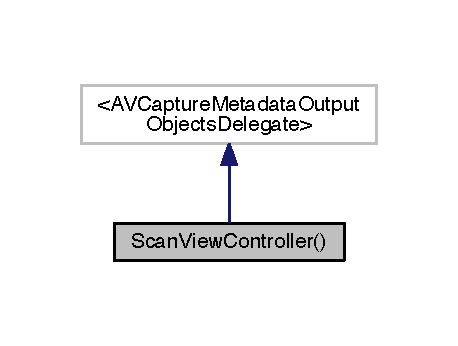
\includegraphics[width=220pt]{category_scan_view_controller_07_08__inherit__graph}
\end{center}
\end{figure}


Collaboration diagram for Scan\+View\+Controller()\+:
\nopagebreak
\begin{figure}[H]
\begin{center}
\leavevmode
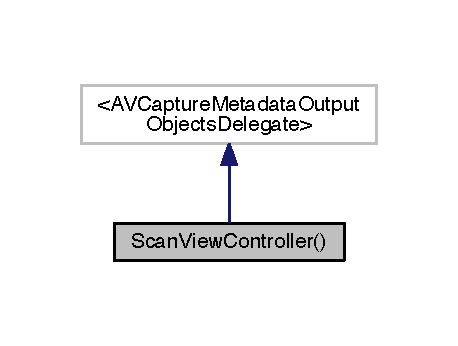
\includegraphics[width=220pt]{category_scan_view_controller_07_08__coll__graph}
\end{center}
\end{figure}
\subsection*{Protected Attributes}
\begin{DoxyCompactItemize}
\item 
A\+V\+Capture\+Session $\ast$ {\bfseries \+\_\+session}\label{category_scan_view_controller_07_08_aaa4b54d43d608a14daff099ca2b5e890}

\item 
A\+V\+Capture\+Device $\ast$ {\bfseries \+\_\+device}\label{category_scan_view_controller_07_08_a8b405bf0c7038a049b8f06da863181f3}

\item 
A\+V\+Capture\+Device\+Input $\ast$ {\bfseries \+\_\+input}\label{category_scan_view_controller_07_08_a13d525b2d8534c27560147b3415080ea}

\item 
A\+V\+Capture\+Metadata\+Output $\ast$ {\bfseries \+\_\+output}\label{category_scan_view_controller_07_08_a458e5f4f769b551dda293364db849e40}

\item 
A\+V\+Capture\+Video\+Preview\+Layer $\ast$ {\bfseries \+\_\+prev\+Layer}\label{category_scan_view_controller_07_08_aae6661ab8758207b3b8a9b39ed9a5edd}

\item 
U\+I\+View $\ast$ {\bfseries \+\_\+highlight\+View}\label{category_scan_view_controller_07_08_a75a7b0ae5ed591056f8a3d351fb35d10}

\item 
U\+I\+Label $\ast$ {\bfseries \+\_\+label}\label{category_scan_view_controller_07_08_a9c46ee545352636c2e8b649a106f7eda}

\end{DoxyCompactItemize}


The documentation for this category was generated from the following file\+:\begin{DoxyCompactItemize}
\item 
Scan\+View\+Controller.\+m\end{DoxyCompactItemize}

\section{Search Class Reference}
\label{interface_search}\index{Search@{Search}}


Inheritance diagram for Search\+:
\nopagebreak
\begin{figure}[H]
\begin{center}
\leavevmode
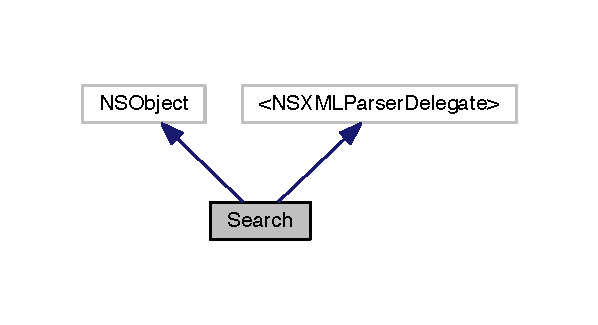
\includegraphics[width=287pt]{interface_search__inherit__graph}
\end{center}
\end{figure}


Collaboration diagram for Search\+:
\nopagebreak
\begin{figure}[H]
\begin{center}
\leavevmode
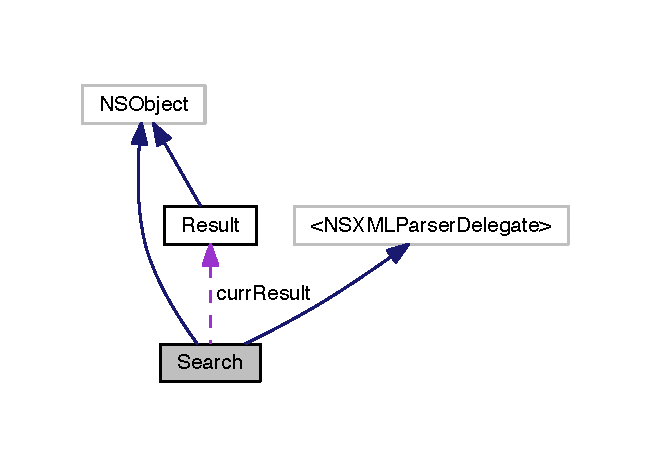
\includegraphics[width=312pt]{interface_search__coll__graph}
\end{center}
\end{figure}
\subsection*{Instance Methods}
\begin{DoxyCompactItemize}
\item 
(void) -\/ {\bfseries find\+Editions}\label{interface_search_af8514e0651d63b7c09faefddb6757dea}

\item 
(void) -\/ {\bfseries find\+Similair}\label{interface_search_a6978268d6c1d71fe36aca04cf6c190f6}

\item 
(N\+S\+Mutable\+Array $\ast$) -\/ {\bfseries get\+Image\+And\+Desc\+::::}\label{interface_search_aa96064736366ce2b85499d0e3800b348}

\item 
(void) -\/ {\bfseries search}\label{interface_search_ae5e5f19a4e800c76823c0781d3cad215}

\item 
(N\+S\+String $\ast$) -\/ {\bfseries check\+I\+S\+B\+N\+:}\label{interface_search_aa221a1145cdaf40c008f25c8ba795e92}

\item 
(Network\+Status) -\/ {\bfseries check\+Connection}\label{interface_search_a296ad648ed932881f08849d95a5d5c95}

\end{DoxyCompactItemize}
\subsection*{Properties}
\begin{DoxyCompactItemize}
\item 
N\+S\+String $\ast$ {\bfseries query}\label{interface_search_aeb04e71a6ca5784a051a7cd63f4e2fc3}

\item 
N\+S\+String $\ast$ {\bfseries query\+Type}\label{interface_search_ac031fcc0b2ce56fb19cdd9694b8cdf2b}

\item 
N\+S\+X\+M\+L\+Parser $\ast$ {\bfseries parser}\label{interface_search_a8e7108974b7159d08459abf52e203827}

\item 
N\+S\+String $\ast$ {\bfseries name}\label{interface_search_ab368ed5b801db165369ebc66c8fafab6}

\item 
{\bf Result} $\ast$ {\bfseries curr\+Result}\label{interface_search_a4e82bb4f5a50ad85a1e2111b012f1a2d}

\item 
N\+S\+Mutable\+Array $\ast$ {\bfseries editions\+I\+S\+B\+N\+S}\label{interface_search_a07ba636aa360e7fb218bf734464861ef}

\item 
N\+S\+Mutable\+Array $\ast$ {\bfseries results}\label{interface_search_a0668886a14e92186615ff6bc00411271}

\item 
N\+S\+Mutable\+Array $\ast$ {\bfseries editions\+Results}\label{interface_search_a3e2691a3fe915d4c9ba857bb4d15263a}

\item 
N\+S\+Mutable\+Array $\ast$ {\bfseries subjects}\label{interface_search_a5b0dd445df4f4e86e71b15f53a609083}

\item 
N\+S\+Mutable\+Array $\ast$ {\bfseries subject\+Results}\label{interface_search_ad219c19b30b84d04cbbd8a5c78a13139}

\item 
N\+S\+Mutable\+Dictionary $\ast$ {\bfseries sim\+Scores}\label{interface_search_a7263d296cac4a23ef4ece7cbfd95aa35}

\item 
N\+S\+String $\ast$ {\bfseries image\+U\+R\+L}\label{interface_search_af1ea0a6d823560bf22ac7ecda4b45189}

\item 
N\+S\+String $\ast$ {\bfseries book\+Desc}\label{interface_search_a5b0aeea3349b499dd87950c5ef889003}

\item 
B\+O\+O\+L {\bfseries did\+Connect}\label{interface_search_a8d9005724e3ac7c89acb6aaf84ed1c0a}

\end{DoxyCompactItemize}


The documentation for this class was generated from the following files\+:\begin{DoxyCompactItemize}
\item 
Search.\+h\item 
Search.\+m\end{DoxyCompactItemize}

\hypertarget{interface_t_f_hpple}{}\section{T\+F\+Hpple Class Reference}
\label{interface_t_f_hpple}\index{T\+F\+Hpple@{T\+F\+Hpple}}


{\ttfamily \#import $<$T\+F\+Hpple.\+h$>$}



Inheritance diagram for T\+F\+Hpple\+:
% FIG 0


Collaboration diagram for T\+F\+Hpple\+:
% FIG 1
\subsection*{Instance Methods}
\begin{DoxyCompactItemize}
\item 
(id) -\/ \hyperlink{interface_t_f_hpple_add58ba26927ae61693fd386325d8f7bb}{init\+With\+Data\+:encoding\+:is\+X\+M\+L\+:}
\item 
(id) -\/ \hyperlink{interface_t_f_hpple_a08f93216c93c656d10f855d0e827bedc}{init\+With\+Data\+:is\+X\+M\+L\+:}
\item 
(id) -\/ \hyperlink{interface_t_f_hpple_a9c736b797fdbbd6b6cd9d0eac9c8115c}{init\+With\+X\+M\+L\+Data\+:encoding\+:}
\item 
(id) -\/ \hyperlink{interface_t_f_hpple_afa3c56c793ee65d94ae60de9162cb375}{init\+With\+X\+M\+L\+Data\+:}
\item 
(id) -\/ \hyperlink{interface_t_f_hpple_a8cb76c8346dde116aeebd11080192368}{init\+With\+H\+T\+M\+L\+Data\+:encoding\+:}
\item 
(id) -\/ \hyperlink{interface_t_f_hpple_a8fecd7b10c51c897d572885daca0b15c}{init\+With\+H\+T\+M\+L\+Data\+:}
\item 
(N\+S\+Array $\ast$) -\/ \hyperlink{interface_t_f_hpple_a5c912f232c2f3b9ef5cf164227ce1016}{search\+With\+X\+Path\+Query\+:}
\item 
(\hyperlink{interface_t_f_hpple_element}{T\+F\+Hpple\+Element} $\ast$) -\/ \hyperlink{interface_t_f_hpple_abe341e921def7fa82a96ed265ce2fd4e}{peek\+At\+Search\+With\+X\+Path\+Query\+:}
\end{DoxyCompactItemize}
\subsection*{Class Methods}
\begin{DoxyCompactItemize}
\item 
(\hyperlink{interface_t_f_hpple}{T\+F\+Hpple} $\ast$) + \hyperlink{interface_t_f_hpple_ae90410d514268088d6c782bb75314523}{hpple\+With\+Data\+:encoding\+:is\+X\+M\+L\+:}
\item 
(\hyperlink{interface_t_f_hpple}{T\+F\+Hpple} $\ast$) + \hyperlink{interface_t_f_hpple_a3a71c0b14f603c7a0c9a51e94b1901db}{hpple\+With\+Data\+:is\+X\+M\+L\+:}
\item 
(\hyperlink{interface_t_f_hpple}{T\+F\+Hpple} $\ast$) + \hyperlink{interface_t_f_hpple_a60815c4d5bbf7d15d1970a63d6c069e9}{hpple\+With\+X\+M\+L\+Data\+:encoding\+:}
\item 
(\hyperlink{interface_t_f_hpple}{T\+F\+Hpple} $\ast$) + \hyperlink{interface_t_f_hpple_a9f6634ba04c1756a00919171cc26ea6b}{hpple\+With\+X\+M\+L\+Data\+:}
\item 
(\hyperlink{interface_t_f_hpple}{T\+F\+Hpple} $\ast$) + \hyperlink{interface_t_f_hpple_ae83067b1e5c80647d2bd1d19d5d391ff}{hpple\+With\+H\+T\+M\+L\+Data\+:encoding\+:}
\item 
(\hyperlink{interface_t_f_hpple}{T\+F\+Hpple} $\ast$) + \hyperlink{interface_t_f_hpple_a05ff6db676283713ae714fcfb9a485a9}{hpple\+With\+H\+T\+M\+L\+Data\+:}
\end{DoxyCompactItemize}
\subsection*{Properties}
\begin{DoxyCompactItemize}
\item 
N\+S\+Data $\ast$ \hyperlink{interface_t_f_hpple_af8002e454472111f4af37d7b48ccbade}{data}
\item 
N\+S\+String $\ast$ \hyperlink{interface_t_f_hpple_a790232945cc92e254fb9788089273d1f}{encoding}
\end{DoxyCompactItemize}


\subsection{Method Documentation}
\hypertarget{interface_t_f_hpple_ae90410d514268088d6c782bb75314523}{}\index{T\+F\+Hpple@{T\+F\+Hpple}!hpple\+With\+Data\+:encoding\+:is\+X\+M\+L\+:@{hpple\+With\+Data\+:encoding\+:is\+X\+M\+L\+:}}
\index{hpple\+With\+Data\+:encoding\+:is\+X\+M\+L\+:@{hpple\+With\+Data\+:encoding\+:is\+X\+M\+L\+:}!T\+F\+Hpple@{T\+F\+Hpple}}
\subsubsection[{hpple\+With\+Data\+:encoding\+:is\+X\+M\+L\+:(\+N\+S\+Data $\ast$the\+Data,[encoding] N\+S\+String $\ast$encoding,[is\+X\+M\+L] B\+O\+O\+L is\+Data\+X\+M\+L)}]{\setlength{\rightskip}{0pt plus 5cm}+ ({\bf T\+F\+Hpple} $\ast$) hpple\+With\+Data\+: 
\begin{DoxyParamCaption}
\item[{(N\+S\+Data $\ast$)}]{the\+Data}
\item[{encoding:(N\+S\+String $\ast$)}]{encoding}
\item[{isXML:(B\+O\+O\+L)}]{is\+Data\+X\+M\+L}
\end{DoxyParamCaption}
}\label{interface_t_f_hpple_ae90410d514268088d6c782bb75314523}
\hypertarget{interface_t_f_hpple_a3a71c0b14f603c7a0c9a51e94b1901db}{}\index{T\+F\+Hpple@{T\+F\+Hpple}!hpple\+With\+Data\+:is\+X\+M\+L\+:@{hpple\+With\+Data\+:is\+X\+M\+L\+:}}
\index{hpple\+With\+Data\+:is\+X\+M\+L\+:@{hpple\+With\+Data\+:is\+X\+M\+L\+:}!T\+F\+Hpple@{T\+F\+Hpple}}
\subsubsection[{hpple\+With\+Data\+:is\+X\+M\+L\+:(\+N\+S\+Data $\ast$the\+Data,[is\+X\+M\+L] B\+O\+O\+L is\+Data\+X\+M\+L)}]{\setlength{\rightskip}{0pt plus 5cm}+ ({\bf T\+F\+Hpple} $\ast$) hpple\+With\+Data\+: 
\begin{DoxyParamCaption}
\item[{(N\+S\+Data $\ast$)}]{the\+Data}
\item[{isXML:(B\+O\+O\+L)}]{is\+Data\+X\+M\+L}
\end{DoxyParamCaption}
}\label{interface_t_f_hpple_a3a71c0b14f603c7a0c9a51e94b1901db}
\hypertarget{interface_t_f_hpple_a05ff6db676283713ae714fcfb9a485a9}{}\index{T\+F\+Hpple@{T\+F\+Hpple}!hpple\+With\+H\+T\+M\+L\+Data\+:@{hpple\+With\+H\+T\+M\+L\+Data\+:}}
\index{hpple\+With\+H\+T\+M\+L\+Data\+:@{hpple\+With\+H\+T\+M\+L\+Data\+:}!T\+F\+Hpple@{T\+F\+Hpple}}
\subsubsection[{hpple\+With\+H\+T\+M\+L\+Data\+:(\+N\+S\+Data $\ast$the\+Data)}]{\setlength{\rightskip}{0pt plus 5cm}+ ({\bf T\+F\+Hpple} $\ast$) hpple\+With\+H\+T\+M\+L\+Data\+: 
\begin{DoxyParamCaption}
\item[{(N\+S\+Data $\ast$)}]{the\+Data}
\end{DoxyParamCaption}
}\label{interface_t_f_hpple_a05ff6db676283713ae714fcfb9a485a9}
\hypertarget{interface_t_f_hpple_ae83067b1e5c80647d2bd1d19d5d391ff}{}\index{T\+F\+Hpple@{T\+F\+Hpple}!hpple\+With\+H\+T\+M\+L\+Data\+:encoding\+:@{hpple\+With\+H\+T\+M\+L\+Data\+:encoding\+:}}
\index{hpple\+With\+H\+T\+M\+L\+Data\+:encoding\+:@{hpple\+With\+H\+T\+M\+L\+Data\+:encoding\+:}!T\+F\+Hpple@{T\+F\+Hpple}}
\subsubsection[{hpple\+With\+H\+T\+M\+L\+Data\+:encoding\+:(\+N\+S\+Data $\ast$the\+Data,[encoding] N\+S\+String $\ast$encoding)}]{\setlength{\rightskip}{0pt plus 5cm}+ ({\bf T\+F\+Hpple} $\ast$) {\bf hpple\+With\+H\+T\+M\+L\+Data\+:} 
\begin{DoxyParamCaption}
\item[{(N\+S\+Data $\ast$)}]{the\+Data}
\item[{encoding:(N\+S\+String $\ast$)}]{encoding}
\end{DoxyParamCaption}
}\label{interface_t_f_hpple_ae83067b1e5c80647d2bd1d19d5d391ff}
\hypertarget{interface_t_f_hpple_a9f6634ba04c1756a00919171cc26ea6b}{}\index{T\+F\+Hpple@{T\+F\+Hpple}!hpple\+With\+X\+M\+L\+Data\+:@{hpple\+With\+X\+M\+L\+Data\+:}}
\index{hpple\+With\+X\+M\+L\+Data\+:@{hpple\+With\+X\+M\+L\+Data\+:}!T\+F\+Hpple@{T\+F\+Hpple}}
\subsubsection[{hpple\+With\+X\+M\+L\+Data\+:(\+N\+S\+Data $\ast$the\+Data)}]{\setlength{\rightskip}{0pt plus 5cm}+ ({\bf T\+F\+Hpple} $\ast$) hpple\+With\+X\+M\+L\+Data\+: 
\begin{DoxyParamCaption}
\item[{(N\+S\+Data $\ast$)}]{the\+Data}
\end{DoxyParamCaption}
}\label{interface_t_f_hpple_a9f6634ba04c1756a00919171cc26ea6b}
\hypertarget{interface_t_f_hpple_a60815c4d5bbf7d15d1970a63d6c069e9}{}\index{T\+F\+Hpple@{T\+F\+Hpple}!hpple\+With\+X\+M\+L\+Data\+:encoding\+:@{hpple\+With\+X\+M\+L\+Data\+:encoding\+:}}
\index{hpple\+With\+X\+M\+L\+Data\+:encoding\+:@{hpple\+With\+X\+M\+L\+Data\+:encoding\+:}!T\+F\+Hpple@{T\+F\+Hpple}}
\subsubsection[{hpple\+With\+X\+M\+L\+Data\+:encoding\+:(\+N\+S\+Data $\ast$the\+Data,[encoding] N\+S\+String $\ast$encoding)}]{\setlength{\rightskip}{0pt plus 5cm}+ ({\bf T\+F\+Hpple} $\ast$) {\bf hpple\+With\+X\+M\+L\+Data\+:} 
\begin{DoxyParamCaption}
\item[{(N\+S\+Data $\ast$)}]{the\+Data}
\item[{encoding:(N\+S\+String $\ast$)}]{encoding}
\end{DoxyParamCaption}
}\label{interface_t_f_hpple_a60815c4d5bbf7d15d1970a63d6c069e9}
\hypertarget{interface_t_f_hpple_add58ba26927ae61693fd386325d8f7bb}{}\index{T\+F\+Hpple@{T\+F\+Hpple}!init\+With\+Data\+:encoding\+:is\+X\+M\+L\+:@{init\+With\+Data\+:encoding\+:is\+X\+M\+L\+:}}
\index{init\+With\+Data\+:encoding\+:is\+X\+M\+L\+:@{init\+With\+Data\+:encoding\+:is\+X\+M\+L\+:}!T\+F\+Hpple@{T\+F\+Hpple}}
\subsubsection[{init\+With\+Data\+:encoding\+:is\+X\+M\+L\+:(\+N\+S\+Data $\ast$the\+Data,[encoding] N\+S\+String $\ast$encoding,[is\+X\+M\+L] B\+O\+O\+L is\+Data\+X\+M\+L)}]{\setlength{\rightskip}{0pt plus 5cm}-\/ (id) init\+With\+Data\+: 
\begin{DoxyParamCaption}
\item[{(N\+S\+Data $\ast$)}]{the\+Data}
\item[{encoding:(N\+S\+String $\ast$)}]{encoding}
\item[{isXML:(B\+O\+O\+L)}]{is\+Data\+X\+M\+L}
\end{DoxyParamCaption}
}\label{interface_t_f_hpple_add58ba26927ae61693fd386325d8f7bb}


Here is the caller graph for this function\+:
% FIG 2


\hypertarget{interface_t_f_hpple_a08f93216c93c656d10f855d0e827bedc}{}\index{T\+F\+Hpple@{T\+F\+Hpple}!init\+With\+Data\+:is\+X\+M\+L\+:@{init\+With\+Data\+:is\+X\+M\+L\+:}}
\index{init\+With\+Data\+:is\+X\+M\+L\+:@{init\+With\+Data\+:is\+X\+M\+L\+:}!T\+F\+Hpple@{T\+F\+Hpple}}
\subsubsection[{init\+With\+Data\+:is\+X\+M\+L\+:(\+N\+S\+Data $\ast$the\+Data,[is\+X\+M\+L] B\+O\+O\+L is\+Data\+X\+M\+L)}]{\setlength{\rightskip}{0pt plus 5cm}-\/ (id) init\+With\+Data\+: 
\begin{DoxyParamCaption}
\item[{(N\+S\+Data $\ast$)}]{the\+Data}
\item[{isXML:(B\+O\+O\+L)}]{is\+Data\+X\+M\+L}
\end{DoxyParamCaption}
}\label{interface_t_f_hpple_a08f93216c93c656d10f855d0e827bedc}


Here is the call graph for this function\+:
% FIG 3


\hypertarget{interface_t_f_hpple_a8fecd7b10c51c897d572885daca0b15c}{}\index{T\+F\+Hpple@{T\+F\+Hpple}!init\+With\+H\+T\+M\+L\+Data\+:@{init\+With\+H\+T\+M\+L\+Data\+:}}
\index{init\+With\+H\+T\+M\+L\+Data\+:@{init\+With\+H\+T\+M\+L\+Data\+:}!T\+F\+Hpple@{T\+F\+Hpple}}
\subsubsection[{init\+With\+H\+T\+M\+L\+Data\+:(\+N\+S\+Data $\ast$the\+Data)}]{\setlength{\rightskip}{0pt plus 5cm}-\/ (id) init\+With\+H\+T\+M\+L\+Data\+: 
\begin{DoxyParamCaption}
\item[{(N\+S\+Data $\ast$)}]{the\+Data}
\end{DoxyParamCaption}
}\label{interface_t_f_hpple_a8fecd7b10c51c897d572885daca0b15c}


Here is the call graph for this function\+:
% FIG 4


\hypertarget{interface_t_f_hpple_a8cb76c8346dde116aeebd11080192368}{}\index{T\+F\+Hpple@{T\+F\+Hpple}!init\+With\+H\+T\+M\+L\+Data\+:encoding\+:@{init\+With\+H\+T\+M\+L\+Data\+:encoding\+:}}
\index{init\+With\+H\+T\+M\+L\+Data\+:encoding\+:@{init\+With\+H\+T\+M\+L\+Data\+:encoding\+:}!T\+F\+Hpple@{T\+F\+Hpple}}
\subsubsection[{init\+With\+H\+T\+M\+L\+Data\+:encoding\+:(\+N\+S\+Data $\ast$the\+Data,[encoding] N\+S\+String $\ast$encoding)}]{\setlength{\rightskip}{0pt plus 5cm}-\/ (id) {\bf init\+With\+H\+T\+M\+L\+Data\+:} 
\begin{DoxyParamCaption}
\item[{(N\+S\+Data $\ast$)}]{the\+Data}
\item[{encoding:(N\+S\+String $\ast$)}]{encoding}
\end{DoxyParamCaption}
}\label{interface_t_f_hpple_a8cb76c8346dde116aeebd11080192368}


Here is the call graph for this function\+:
% FIG 5


\hypertarget{interface_t_f_hpple_afa3c56c793ee65d94ae60de9162cb375}{}\index{T\+F\+Hpple@{T\+F\+Hpple}!init\+With\+X\+M\+L\+Data\+:@{init\+With\+X\+M\+L\+Data\+:}}
\index{init\+With\+X\+M\+L\+Data\+:@{init\+With\+X\+M\+L\+Data\+:}!T\+F\+Hpple@{T\+F\+Hpple}}
\subsubsection[{init\+With\+X\+M\+L\+Data\+:(\+N\+S\+Data $\ast$the\+Data)}]{\setlength{\rightskip}{0pt plus 5cm}-\/ (id) init\+With\+X\+M\+L\+Data\+: 
\begin{DoxyParamCaption}
\item[{(N\+S\+Data $\ast$)}]{the\+Data}
\end{DoxyParamCaption}
}\label{interface_t_f_hpple_afa3c56c793ee65d94ae60de9162cb375}


Here is the call graph for this function\+:
% FIG 6


\hypertarget{interface_t_f_hpple_a9c736b797fdbbd6b6cd9d0eac9c8115c}{}\index{T\+F\+Hpple@{T\+F\+Hpple}!init\+With\+X\+M\+L\+Data\+:encoding\+:@{init\+With\+X\+M\+L\+Data\+:encoding\+:}}
\index{init\+With\+X\+M\+L\+Data\+:encoding\+:@{init\+With\+X\+M\+L\+Data\+:encoding\+:}!T\+F\+Hpple@{T\+F\+Hpple}}
\subsubsection[{init\+With\+X\+M\+L\+Data\+:encoding\+:(\+N\+S\+Data $\ast$the\+Data,[encoding] N\+S\+String $\ast$encoding)}]{\setlength{\rightskip}{0pt plus 5cm}-\/ (id) {\bf init\+With\+X\+M\+L\+Data\+:} 
\begin{DoxyParamCaption}
\item[{(N\+S\+Data $\ast$)}]{the\+Data}
\item[{encoding:(N\+S\+String $\ast$)}]{encoding}
\end{DoxyParamCaption}
}\label{interface_t_f_hpple_a9c736b797fdbbd6b6cd9d0eac9c8115c}


Here is the call graph for this function\+:
% FIG 7


\hypertarget{interface_t_f_hpple_abe341e921def7fa82a96ed265ce2fd4e}{}\index{T\+F\+Hpple@{T\+F\+Hpple}!peek\+At\+Search\+With\+X\+Path\+Query\+:@{peek\+At\+Search\+With\+X\+Path\+Query\+:}}
\index{peek\+At\+Search\+With\+X\+Path\+Query\+:@{peek\+At\+Search\+With\+X\+Path\+Query\+:}!T\+F\+Hpple@{T\+F\+Hpple}}
\subsubsection[{peek\+At\+Search\+With\+X\+Path\+Query\+:(\+N\+S\+String $\ast$x\+Path\+Or\+C\+S\+S)}]{\setlength{\rightskip}{0pt plus 5cm}-\/ ({\bf T\+F\+Hpple\+Element} $\ast$) peek\+At\+Search\+With\+X\+Path\+Query\+: 
\begin{DoxyParamCaption}
\item[{(N\+S\+String $\ast$)}]{x\+Path\+Or\+C\+S\+S}
\end{DoxyParamCaption}
}\label{interface_t_f_hpple_abe341e921def7fa82a96ed265ce2fd4e}


Here is the call graph for this function\+:
% FIG 8


\hypertarget{interface_t_f_hpple_a5c912f232c2f3b9ef5cf164227ce1016}{}\index{T\+F\+Hpple@{T\+F\+Hpple}!search\+With\+X\+Path\+Query\+:@{search\+With\+X\+Path\+Query\+:}}
\index{search\+With\+X\+Path\+Query\+:@{search\+With\+X\+Path\+Query\+:}!T\+F\+Hpple@{T\+F\+Hpple}}
\subsubsection[{search\+With\+X\+Path\+Query\+:(\+N\+S\+String $\ast$x\+Path\+Or\+C\+S\+S)}]{\setlength{\rightskip}{0pt plus 5cm}-\/ (N\+S\+Array $\ast$) search\+With\+X\+Path\+Query\+: 
\begin{DoxyParamCaption}
\item[{(N\+S\+String $\ast$)}]{x\+Path\+Or\+C\+S\+S}
\end{DoxyParamCaption}
}\label{interface_t_f_hpple_a5c912f232c2f3b9ef5cf164227ce1016}


Here is the call graph for this function\+:
% FIG 9




Here is the caller graph for this function\+:
% FIG 10




\subsection{Property Documentation}
\hypertarget{interface_t_f_hpple_af8002e454472111f4af37d7b48ccbade}{}\index{T\+F\+Hpple@{T\+F\+Hpple}!data@{data}}
\index{data@{data}!T\+F\+Hpple@{T\+F\+Hpple}}
\subsubsection[{data}]{\setlength{\rightskip}{0pt plus 5cm}-\/ (N\+S\+Data$\ast$) data\hspace{0.3cm}{\ttfamily [read]}, {\ttfamily [nonatomic]}, {\ttfamily [assign]}}\label{interface_t_f_hpple_af8002e454472111f4af37d7b48ccbade}
\hypertarget{interface_t_f_hpple_a790232945cc92e254fb9788089273d1f}{}\index{T\+F\+Hpple@{T\+F\+Hpple}!encoding@{encoding}}
\index{encoding@{encoding}!T\+F\+Hpple@{T\+F\+Hpple}}
\subsubsection[{encoding}]{\setlength{\rightskip}{0pt plus 5cm}-\/ (N\+S\+String$\ast$) encoding\hspace{0.3cm}{\ttfamily [read]}, {\ttfamily [nonatomic]}, {\ttfamily [assign]}}\label{interface_t_f_hpple_a790232945cc92e254fb9788089273d1f}


The documentation for this class was generated from the following files\+:\begin{DoxyCompactItemize}
\item 
Library\+Books/\hyperlink{_t_f_hpple_8h}{T\+F\+Hpple.\+h}\item 
Library\+Books/\hyperlink{_t_f_hpple_8m}{T\+F\+Hpple.\+m}\end{DoxyCompactItemize}

\section{T\+F\+Hpple() Category Reference}
\label{category_t_f_hpple_07_08}\index{T\+F\+Hpple()@{T\+F\+Hpple()}}
\subsection*{Protected Attributes}
\begin{DoxyCompactItemize}
\item 
N\+S\+Data $\ast$ {\bfseries data}\label{category_t_f_hpple_07_08_a674b2440c6e918dcf6b323786bd29ecb}

\item 
N\+S\+String $\ast$ {\bfseries encoding}\label{category_t_f_hpple_07_08_a0b3df7514a4fe4565450e3a19f390e0a}

\item 
B\+O\+O\+L {\bfseries is\+X\+M\+L}\label{category_t_f_hpple_07_08_ad2ae7e483fc2540b363e72a46a4cb196}

\end{DoxyCompactItemize}


The documentation for this category was generated from the following file\+:\begin{DoxyCompactItemize}
\item 
T\+F\+Hpple.\+m\end{DoxyCompactItemize}

\hypertarget{interface_t_f_hpple_element}{}\section{T\+F\+Hpple\+Element Class Reference}
\label{interface_t_f_hpple_element}\index{T\+F\+Hpple\+Element@{T\+F\+Hpple\+Element}}


{\ttfamily \#import $<$T\+F\+Hpple\+Element.\+h$>$}



Inheritance diagram for T\+F\+Hpple\+Element\+:
% FIG 0


Collaboration diagram for T\+F\+Hpple\+Element\+:
% FIG 1
\subsection*{Instance Methods}
\begin{DoxyCompactItemize}
\item 
(id) -\/ \hyperlink{interface_t_f_hpple_element_a96f0b88ecc6a2d995db83adc29c651a0}{init\+With\+Node\+:is\+X\+M\+L\+:with\+Encoding\+:}
\item 
(B\+O\+O\+L) -\/ \hyperlink{interface_t_f_hpple_element_ad3bc62dda4b012f0fa3db18de0fc4bdb}{has\+Children}
\item 
(B\+O\+O\+L) -\/ \hyperlink{interface_t_f_hpple_element_aa8dfd3d004a8426a8768d0b9895be6c8}{is\+Text\+Node}
\item 
(N\+S\+String $\ast$) -\/ \hyperlink{interface_t_f_hpple_element_aed2c4dacaa682b1922bb04ef4aa44994}{object\+For\+Key\+:}
\item 
(N\+S\+Array $\ast$) -\/ \hyperlink{interface_t_f_hpple_element_a4ec6f4d6b0cb04ed9a19c392226034bd}{children\+With\+Tag\+Name\+:}
\item 
(\hyperlink{interface_t_f_hpple_element}{T\+F\+Hpple\+Element} $\ast$) -\/ \hyperlink{interface_t_f_hpple_element_a54c3359b7e1ca0bca26c4e6ff0473c9b}{first\+Child\+With\+Tag\+Name\+:}
\item 
(N\+S\+Array $\ast$) -\/ \hyperlink{interface_t_f_hpple_element_a33bda9b36b3a6b6cb8aa3191e4d8081d}{children\+With\+Class\+Name\+:}
\item 
(\hyperlink{interface_t_f_hpple_element}{T\+F\+Hpple\+Element} $\ast$) -\/ \hyperlink{interface_t_f_hpple_element_ae19ca4aaac4865f61f02e81869394c76}{first\+Child\+With\+Class\+Name\+:}
\item 
(\hyperlink{interface_t_f_hpple_element}{T\+F\+Hpple\+Element} $\ast$) -\/ \hyperlink{interface_t_f_hpple_element_a73a7c62150c93492a29364763a0e2704}{first\+Text\+Child}
\item 
(N\+S\+String $\ast$) -\/ \hyperlink{interface_t_f_hpple_element_a45cde91bb698bdbb03f4c48a896b031a}{text}
\item 
(N\+S\+Array $\ast$) -\/ \hyperlink{interface_t_f_hpple_element_af82deb9f4a9a92339829b9bab17ab9b9}{search\+With\+X\+Path\+Query\+:}
\item 
(id) -\/ \hyperlink{interface_t_f_hpple_element_ae1c9cc9af79c5a5b41d19188444a43f7}{object\+For\+Keyed\+Subscript\+:}
\end{DoxyCompactItemize}
\subsection*{Class Methods}
\begin{DoxyCompactItemize}
\item 
(\hyperlink{interface_t_f_hpple_element}{T\+F\+Hpple\+Element} $\ast$) + \hyperlink{interface_t_f_hpple_element_a617d6eb7c9674ebfced840c1764028a5}{hpple\+Element\+With\+Node\+:is\+X\+M\+L\+:with\+Encoding\+:}
\end{DoxyCompactItemize}
\subsection*{Properties}
\begin{DoxyCompactItemize}
\item 
N\+S\+String $\ast$ \hyperlink{interface_t_f_hpple_element_a67a2f29f7e31c69d23e2365f7602241a}{raw}
\item 
N\+S\+String $\ast$ \hyperlink{interface_t_f_hpple_element_a92efb1ac82fa89fe4221a7f2363332ea}{content}
\item 
N\+S\+String $\ast$ \hyperlink{interface_t_f_hpple_element_a25cfdaa376701dc9817c1b2c7e135b75}{tag\+Name}
\item 
N\+S\+Dictionary $\ast$ \hyperlink{interface_t_f_hpple_element_aea9972700f45beb7197f03b20cfbd3d2}{attributes}
\item 
N\+S\+Array $\ast$ \hyperlink{interface_t_f_hpple_element_a6023a02b0f33943aad395504981b24ba}{children}
\item 
\hyperlink{interface_t_f_hpple_element}{T\+F\+Hpple\+Element} $\ast$ \hyperlink{interface_t_f_hpple_element_afb83964b315f36faa2ad67dc71645ada}{first\+Child}
\item 
\hyperlink{interface_t_f_hpple_element}{T\+F\+Hpple\+Element} $\ast$ \hyperlink{interface_t_f_hpple_element_a8fc33c0ff70941d9638f05632ad6ba5d}{parent}
\end{DoxyCompactItemize}


\subsection{Method Documentation}
\hypertarget{interface_t_f_hpple_element_a33bda9b36b3a6b6cb8aa3191e4d8081d}{}\index{T\+F\+Hpple\+Element@{T\+F\+Hpple\+Element}!children\+With\+Class\+Name\+:@{children\+With\+Class\+Name\+:}}
\index{children\+With\+Class\+Name\+:@{children\+With\+Class\+Name\+:}!T\+F\+Hpple\+Element@{T\+F\+Hpple\+Element}}
\subsubsection[{children\+With\+Class\+Name\+:(\+N\+S\+String $\ast$class\+Name)}]{\setlength{\rightskip}{0pt plus 5cm}-\/ (N\+S\+Array $\ast$) children\+With\+Class\+Name\+: 
\begin{DoxyParamCaption}
\item[{(N\+S\+String $\ast$)}]{class\+Name}
\end{DoxyParamCaption}
}\label{interface_t_f_hpple_element_a33bda9b36b3a6b6cb8aa3191e4d8081d}
\hypertarget{interface_t_f_hpple_element_a4ec6f4d6b0cb04ed9a19c392226034bd}{}\index{T\+F\+Hpple\+Element@{T\+F\+Hpple\+Element}!children\+With\+Tag\+Name\+:@{children\+With\+Tag\+Name\+:}}
\index{children\+With\+Tag\+Name\+:@{children\+With\+Tag\+Name\+:}!T\+F\+Hpple\+Element@{T\+F\+Hpple\+Element}}
\subsubsection[{children\+With\+Tag\+Name\+:(\+N\+S\+String $\ast$tag\+Name)}]{\setlength{\rightskip}{0pt plus 5cm}-\/ (N\+S\+Array $\ast$) children\+With\+Tag\+Name\+: 
\begin{DoxyParamCaption}
\item[{(N\+S\+String $\ast$)}]{tag\+Name}
\end{DoxyParamCaption}
}\label{interface_t_f_hpple_element_a4ec6f4d6b0cb04ed9a19c392226034bd}
\hypertarget{interface_t_f_hpple_element_ae19ca4aaac4865f61f02e81869394c76}{}\index{T\+F\+Hpple\+Element@{T\+F\+Hpple\+Element}!first\+Child\+With\+Class\+Name\+:@{first\+Child\+With\+Class\+Name\+:}}
\index{first\+Child\+With\+Class\+Name\+:@{first\+Child\+With\+Class\+Name\+:}!T\+F\+Hpple\+Element@{T\+F\+Hpple\+Element}}
\subsubsection[{first\+Child\+With\+Class\+Name\+:(\+N\+S\+String $\ast$class\+Name)}]{\setlength{\rightskip}{0pt plus 5cm}-\/ ({\bf T\+F\+Hpple\+Element} $\ast$) first\+Child\+With\+Class\+Name\+: 
\begin{DoxyParamCaption}
\item[{(N\+S\+String$\ast$)}]{class\+Name}
\end{DoxyParamCaption}
}\label{interface_t_f_hpple_element_ae19ca4aaac4865f61f02e81869394c76}
\hypertarget{interface_t_f_hpple_element_a54c3359b7e1ca0bca26c4e6ff0473c9b}{}\index{T\+F\+Hpple\+Element@{T\+F\+Hpple\+Element}!first\+Child\+With\+Tag\+Name\+:@{first\+Child\+With\+Tag\+Name\+:}}
\index{first\+Child\+With\+Tag\+Name\+:@{first\+Child\+With\+Tag\+Name\+:}!T\+F\+Hpple\+Element@{T\+F\+Hpple\+Element}}
\subsubsection[{first\+Child\+With\+Tag\+Name\+:(\+N\+S\+String $\ast$tag\+Name)}]{\setlength{\rightskip}{0pt plus 5cm}-\/ ({\bf T\+F\+Hpple\+Element} $\ast$) first\+Child\+With\+Tag\+Name\+: 
\begin{DoxyParamCaption}
\item[{(N\+S\+String $\ast$)}]{tag\+Name}
\end{DoxyParamCaption}
}\label{interface_t_f_hpple_element_a54c3359b7e1ca0bca26c4e6ff0473c9b}


Here is the caller graph for this function\+:
% FIG 2


\hypertarget{interface_t_f_hpple_element_a73a7c62150c93492a29364763a0e2704}{}\index{T\+F\+Hpple\+Element@{T\+F\+Hpple\+Element}!first\+Text\+Child@{first\+Text\+Child}}
\index{first\+Text\+Child@{first\+Text\+Child}!T\+F\+Hpple\+Element@{T\+F\+Hpple\+Element}}
\subsubsection[{first\+Text\+Child()}]{\setlength{\rightskip}{0pt plus 5cm}-\/ ({\bf T\+F\+Hpple\+Element} $\ast$) first\+Text\+Child 
\begin{DoxyParamCaption}
{}
\end{DoxyParamCaption}
}\label{interface_t_f_hpple_element_a73a7c62150c93492a29364763a0e2704}


Here is the call graph for this function\+:
% FIG 3


\hypertarget{interface_t_f_hpple_element_ad3bc62dda4b012f0fa3db18de0fc4bdb}{}\index{T\+F\+Hpple\+Element@{T\+F\+Hpple\+Element}!has\+Children@{has\+Children}}
\index{has\+Children@{has\+Children}!T\+F\+Hpple\+Element@{T\+F\+Hpple\+Element}}
\subsubsection[{has\+Children()}]{\setlength{\rightskip}{0pt plus 5cm}-\/ (B\+O\+O\+L) has\+Children 
\begin{DoxyParamCaption}
{}
\end{DoxyParamCaption}
}\label{interface_t_f_hpple_element_ad3bc62dda4b012f0fa3db18de0fc4bdb}
\hypertarget{interface_t_f_hpple_element_a617d6eb7c9674ebfced840c1764028a5}{}\index{T\+F\+Hpple\+Element@{T\+F\+Hpple\+Element}!hpple\+Element\+With\+Node\+:is\+X\+M\+L\+:with\+Encoding\+:@{hpple\+Element\+With\+Node\+:is\+X\+M\+L\+:with\+Encoding\+:}}
\index{hpple\+Element\+With\+Node\+:is\+X\+M\+L\+:with\+Encoding\+:@{hpple\+Element\+With\+Node\+:is\+X\+M\+L\+:with\+Encoding\+:}!T\+F\+Hpple\+Element@{T\+F\+Hpple\+Element}}
\subsubsection[{hpple\+Element\+With\+Node\+:is\+X\+M\+L\+:with\+Encoding\+:(\+N\+S\+Dictionary $\ast$the\+Node,[is\+X\+M\+L] B\+O\+O\+L is\+Data\+X\+M\+L,[with\+Encoding] N\+S\+String $\ast$the\+Encoding)}]{\setlength{\rightskip}{0pt plus 5cm}+ ({\bf T\+F\+Hpple\+Element} $\ast$) hpple\+Element\+With\+Node\+: 
\begin{DoxyParamCaption}
\item[{(N\+S\+Dictionary $\ast$)}]{the\+Node}
\item[{isXML:(B\+O\+O\+L)}]{is\+Data\+X\+M\+L}
\item[{withEncoding:(N\+S\+String $\ast$)}]{the\+Encoding}
\end{DoxyParamCaption}
}\label{interface_t_f_hpple_element_a617d6eb7c9674ebfced840c1764028a5}


Here is the caller graph for this function\+:
% FIG 4


\hypertarget{interface_t_f_hpple_element_a96f0b88ecc6a2d995db83adc29c651a0}{}\index{T\+F\+Hpple\+Element@{T\+F\+Hpple\+Element}!init\+With\+Node\+:is\+X\+M\+L\+:with\+Encoding\+:@{init\+With\+Node\+:is\+X\+M\+L\+:with\+Encoding\+:}}
\index{init\+With\+Node\+:is\+X\+M\+L\+:with\+Encoding\+:@{init\+With\+Node\+:is\+X\+M\+L\+:with\+Encoding\+:}!T\+F\+Hpple\+Element@{T\+F\+Hpple\+Element}}
\subsubsection[{init\+With\+Node\+:is\+X\+M\+L\+:with\+Encoding\+:(\+N\+S\+Dictionary $\ast$the\+Node,[is\+X\+M\+L] B\+O\+O\+L is\+Data\+X\+M\+L,[with\+Encoding] N\+S\+String $\ast$the\+Encoding)}]{\setlength{\rightskip}{0pt plus 5cm}-\/ (id) init\+With\+Node\+: 
\begin{DoxyParamCaption}
\item[{(N\+S\+Dictionary $\ast$)}]{the\+Node}
\item[{isXML:(B\+O\+O\+L)}]{is\+Data\+X\+M\+L}
\item[{withEncoding:(N\+S\+String $\ast$)}]{the\+Encoding}
\end{DoxyParamCaption}
}\label{interface_t_f_hpple_element_a96f0b88ecc6a2d995db83adc29c651a0}
\hypertarget{interface_t_f_hpple_element_aa8dfd3d004a8426a8768d0b9895be6c8}{}\index{T\+F\+Hpple\+Element@{T\+F\+Hpple\+Element}!is\+Text\+Node@{is\+Text\+Node}}
\index{is\+Text\+Node@{is\+Text\+Node}!T\+F\+Hpple\+Element@{T\+F\+Hpple\+Element}}
\subsubsection[{is\+Text\+Node()}]{\setlength{\rightskip}{0pt plus 5cm}-\/ (B\+O\+O\+L) is\+Text\+Node 
\begin{DoxyParamCaption}
{}
\end{DoxyParamCaption}
}\label{interface_t_f_hpple_element_aa8dfd3d004a8426a8768d0b9895be6c8}


Here is the caller graph for this function\+:
% FIG 5


\hypertarget{interface_t_f_hpple_element_aed2c4dacaa682b1922bb04ef4aa44994}{}\index{T\+F\+Hpple\+Element@{T\+F\+Hpple\+Element}!object\+For\+Key\+:@{object\+For\+Key\+:}}
\index{object\+For\+Key\+:@{object\+For\+Key\+:}!T\+F\+Hpple\+Element@{T\+F\+Hpple\+Element}}
\subsubsection[{object\+For\+Key\+:(\+N\+S\+String $\ast$the\+Key)}]{\setlength{\rightskip}{0pt plus 5cm}-\/ (N\+S\+String $\ast$) object\+For\+Key\+: 
\begin{DoxyParamCaption}
\item[{(N\+S\+String $\ast$)}]{the\+Key}
\end{DoxyParamCaption}
}\label{interface_t_f_hpple_element_aed2c4dacaa682b1922bb04ef4aa44994}


Here is the caller graph for this function\+:
% FIG 6


\hypertarget{interface_t_f_hpple_element_ae1c9cc9af79c5a5b41d19188444a43f7}{}\index{T\+F\+Hpple\+Element@{T\+F\+Hpple\+Element}!object\+For\+Keyed\+Subscript\+:@{object\+For\+Keyed\+Subscript\+:}}
\index{object\+For\+Keyed\+Subscript\+:@{object\+For\+Keyed\+Subscript\+:}!T\+F\+Hpple\+Element@{T\+F\+Hpple\+Element}}
\subsubsection[{object\+For\+Keyed\+Subscript\+:(id key)}]{\setlength{\rightskip}{0pt plus 5cm}-\/ (id) object\+For\+Keyed\+Subscript\+: 
\begin{DoxyParamCaption}
\item[{(id)}]{key}
\end{DoxyParamCaption}
}\label{interface_t_f_hpple_element_ae1c9cc9af79c5a5b41d19188444a43f7}


Here is the call graph for this function\+:
% FIG 7


\hypertarget{interface_t_f_hpple_element_af82deb9f4a9a92339829b9bab17ab9b9}{}\index{T\+F\+Hpple\+Element@{T\+F\+Hpple\+Element}!search\+With\+X\+Path\+Query\+:@{search\+With\+X\+Path\+Query\+:}}
\index{search\+With\+X\+Path\+Query\+:@{search\+With\+X\+Path\+Query\+:}!T\+F\+Hpple\+Element@{T\+F\+Hpple\+Element}}
\subsubsection[{search\+With\+X\+Path\+Query\+:(\+N\+S\+String $\ast$x\+Path\+Or\+C\+S\+S)}]{\setlength{\rightskip}{0pt plus 5cm}-\/ (N\+S\+Array $\ast$) search\+With\+X\+Path\+Query\+: 
\begin{DoxyParamCaption}
\item[{(N\+S\+String $\ast$)}]{x\+Path\+Or\+C\+S\+S}
\end{DoxyParamCaption}
}\label{interface_t_f_hpple_element_af82deb9f4a9a92339829b9bab17ab9b9}


Here is the call graph for this function\+:
% FIG 8


\hypertarget{interface_t_f_hpple_element_a45cde91bb698bdbb03f4c48a896b031a}{}\index{T\+F\+Hpple\+Element@{T\+F\+Hpple\+Element}!text@{text}}
\index{text@{text}!T\+F\+Hpple\+Element@{T\+F\+Hpple\+Element}}
\subsubsection[{text()}]{\setlength{\rightskip}{0pt plus 5cm}-\/ (N\+S\+String $\ast$) text 
\begin{DoxyParamCaption}
{}
\end{DoxyParamCaption}
}\label{interface_t_f_hpple_element_a45cde91bb698bdbb03f4c48a896b031a}


\subsection{Property Documentation}
\hypertarget{interface_t_f_hpple_element_aea9972700f45beb7197f03b20cfbd3d2}{}\index{T\+F\+Hpple\+Element@{T\+F\+Hpple\+Element}!attributes@{attributes}}
\index{attributes@{attributes}!T\+F\+Hpple\+Element@{T\+F\+Hpple\+Element}}
\subsubsection[{attributes}]{\setlength{\rightskip}{0pt plus 5cm}-\/ (N\+S\+Dictionary $\ast$) attributes\hspace{0.3cm}{\ttfamily [read]}, {\ttfamily [nonatomic]}, {\ttfamily [strong]}}\label{interface_t_f_hpple_element_aea9972700f45beb7197f03b20cfbd3d2}
\hypertarget{interface_t_f_hpple_element_a6023a02b0f33943aad395504981b24ba}{}\index{T\+F\+Hpple\+Element@{T\+F\+Hpple\+Element}!children@{children}}
\index{children@{children}!T\+F\+Hpple\+Element@{T\+F\+Hpple\+Element}}
\subsubsection[{children}]{\setlength{\rightskip}{0pt plus 5cm}-\/ (N\+S\+Array $\ast$) children\hspace{0.3cm}{\ttfamily [read]}, {\ttfamily [nonatomic]}, {\ttfamily [strong]}}\label{interface_t_f_hpple_element_a6023a02b0f33943aad395504981b24ba}
\hypertarget{interface_t_f_hpple_element_a92efb1ac82fa89fe4221a7f2363332ea}{}\index{T\+F\+Hpple\+Element@{T\+F\+Hpple\+Element}!content@{content}}
\index{content@{content}!T\+F\+Hpple\+Element@{T\+F\+Hpple\+Element}}
\subsubsection[{content}]{\setlength{\rightskip}{0pt plus 5cm}-\/ (N\+S\+String $\ast$) content\hspace{0.3cm}{\ttfamily [read]}, {\ttfamily [nonatomic]}, {\ttfamily [copy]}}\label{interface_t_f_hpple_element_a92efb1ac82fa89fe4221a7f2363332ea}
\hypertarget{interface_t_f_hpple_element_afb83964b315f36faa2ad67dc71645ada}{}\index{T\+F\+Hpple\+Element@{T\+F\+Hpple\+Element}!first\+Child@{first\+Child}}
\index{first\+Child@{first\+Child}!T\+F\+Hpple\+Element@{T\+F\+Hpple\+Element}}
\subsubsection[{first\+Child}]{\setlength{\rightskip}{0pt plus 5cm}-\/ ({\bf T\+F\+Hpple\+Element} $\ast$) first\+Child\hspace{0.3cm}{\ttfamily [read]}, {\ttfamily [nonatomic]}, {\ttfamily [strong]}}\label{interface_t_f_hpple_element_afb83964b315f36faa2ad67dc71645ada}
\hypertarget{interface_t_f_hpple_element_a8fc33c0ff70941d9638f05632ad6ba5d}{}\index{T\+F\+Hpple\+Element@{T\+F\+Hpple\+Element}!parent@{parent}}
\index{parent@{parent}!T\+F\+Hpple\+Element@{T\+F\+Hpple\+Element}}
\subsubsection[{parent}]{\setlength{\rightskip}{0pt plus 5cm}-\/ ({\bf T\+F\+Hpple\+Element}$\ast$) parent\hspace{0.3cm}{\ttfamily [read]}, {\ttfamily [nonatomic]}, {\ttfamily [unsafe_unretained]}}\label{interface_t_f_hpple_element_a8fc33c0ff70941d9638f05632ad6ba5d}
\hypertarget{interface_t_f_hpple_element_a67a2f29f7e31c69d23e2365f7602241a}{}\index{T\+F\+Hpple\+Element@{T\+F\+Hpple\+Element}!raw@{raw}}
\index{raw@{raw}!T\+F\+Hpple\+Element@{T\+F\+Hpple\+Element}}
\subsubsection[{raw}]{\setlength{\rightskip}{0pt plus 5cm}-\/ (N\+S\+String $\ast$) raw\hspace{0.3cm}{\ttfamily [read]}, {\ttfamily [nonatomic]}, {\ttfamily [copy]}}\label{interface_t_f_hpple_element_a67a2f29f7e31c69d23e2365f7602241a}
\hypertarget{interface_t_f_hpple_element_a25cfdaa376701dc9817c1b2c7e135b75}{}\index{T\+F\+Hpple\+Element@{T\+F\+Hpple\+Element}!tag\+Name@{tag\+Name}}
\index{tag\+Name@{tag\+Name}!T\+F\+Hpple\+Element@{T\+F\+Hpple\+Element}}
\subsubsection[{tag\+Name}]{\setlength{\rightskip}{0pt plus 5cm}-\/ (N\+S\+String $\ast$) tag\+Name\hspace{0.3cm}{\ttfamily [read]}, {\ttfamily [nonatomic]}, {\ttfamily [copy]}}\label{interface_t_f_hpple_element_a25cfdaa376701dc9817c1b2c7e135b75}


The documentation for this class was generated from the following files\+:\begin{DoxyCompactItemize}
\item 
Library\+Books/\hyperlink{_t_f_hpple_element_8h}{T\+F\+Hpple\+Element.\+h}\item 
Library\+Books/\hyperlink{_t_f_hpple_element_8m}{T\+F\+Hpple\+Element.\+m}\end{DoxyCompactItemize}

\section{T\+F\+Hpple\+Element() Category Reference}
\label{category_t_f_hpple_element_07_08}\index{T\+F\+Hpple\+Element()@{T\+F\+Hpple\+Element()}}


Collaboration diagram for T\+F\+Hpple\+Element()\+:
\nopagebreak
\begin{figure}[H]
\begin{center}
\leavevmode
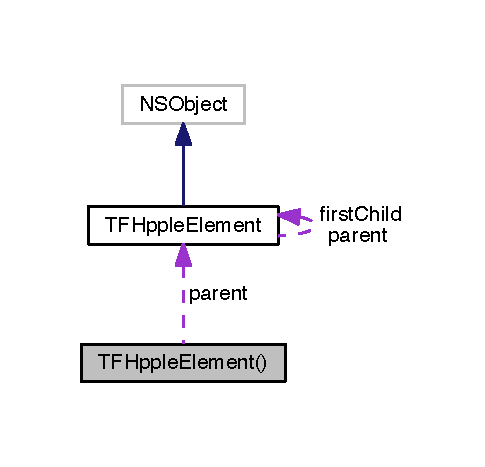
\includegraphics[width=233pt]{category_t_f_hpple_element_07_08__coll__graph}
\end{center}
\end{figure}
\subsection*{Protected Attributes}
\begin{DoxyCompactItemize}
\item 
N\+S\+Dictionary $\ast$ {\bfseries node}\label{category_t_f_hpple_element_07_08_a3742b005d3fd31acacff0d1573cb8a89}

\item 
B\+O\+O\+L {\bfseries is\+X\+M\+L}\label{category_t_f_hpple_element_07_08_a41941751fd0f1fdf6c18c0f90c5991cb}

\item 
N\+S\+String $\ast$ {\bfseries encoding}\label{category_t_f_hpple_element_07_08_a0a7ccc47e17245385fbaf177baad31bf}

\item 
\+\_\+\+\_\+unsafe\+\_\+unretained {\bf T\+F\+Hpple\+Element} $\ast$ {\bfseries parent}\label{category_t_f_hpple_element_07_08_ac7602bad8a05294a6beecabe01e6e569}

\end{DoxyCompactItemize}
\subsection*{Properties}
\begin{DoxyCompactItemize}
\item 
{\bf T\+F\+Hpple\+Element} $\ast$ {\bfseries parent}\label{category_t_f_hpple_element_07_08_a3a570a7692ac21f8d4adc52b4c96756c}

\end{DoxyCompactItemize}


The documentation for this category was generated from the following file\+:\begin{DoxyCompactItemize}
\item 
T\+F\+Hpple\+Element.\+m\end{DoxyCompactItemize}

\section{web\+View\+Controller Class Reference}
\label{interfaceweb_view_controller}\index{web\+View\+Controller@{web\+View\+Controller}}


Inheritance diagram for web\+View\+Controller\+:
\nopagebreak
\begin{figure}[H]
\begin{center}
\leavevmode
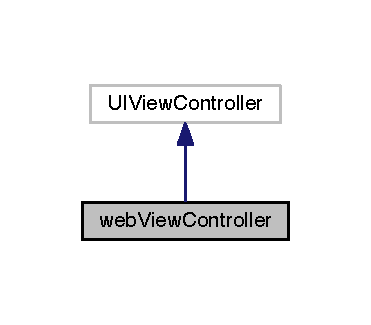
\includegraphics[width=178pt]{interfaceweb_view_controller__inherit__graph}
\end{center}
\end{figure}


Collaboration diagram for web\+View\+Controller\+:
\nopagebreak
\begin{figure}[H]
\begin{center}
\leavevmode
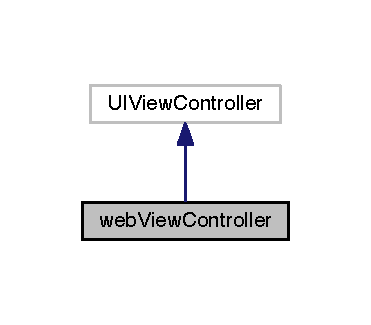
\includegraphics[width=178pt]{interfaceweb_view_controller__coll__graph}
\end{center}
\end{figure}
\subsection*{Properties}
\begin{DoxyCompactItemize}
\item 
I\+B\+Outlet U\+I\+Activity\+Indicator\+View $\ast$ {\bfseries load\+Indicator}\label{interfaceweb_view_controller_aed50ed21f737cd77446aca759e3ab5a7}

\item 
I\+B\+Outlet U\+I\+Web\+View $\ast$ {\bfseries web\+Page}\label{interfaceweb_view_controller_a0a973d91b25a215ef7df7b9e5e6ad860}

\item 
N\+S\+String $\ast$ {\bfseries url}\label{interfaceweb_view_controller_a6b63e34b44fea86498e7c602ee3700a9}

\end{DoxyCompactItemize}


The documentation for this class was generated from the following file\+:\begin{DoxyCompactItemize}
\item 
web\+View\+Controller.\+h\end{DoxyCompactItemize}

\section{web\+View\+Controller() Category Reference}
\label{categoryweb_view_controller_07_08}\index{web\+View\+Controller()@{web\+View\+Controller()}}


The documentation for this category was generated from the following file\+:\begin{DoxyCompactItemize}
\item 
web\+View\+Controller.\+m\end{DoxyCompactItemize}

%--- End generated contents ---

% Index
\backmatter
\newpage
\phantomsection
\clearemptydoublepage
\addcontentsline{toc}{chapter}{Index}
\printindex

\end{document}
